
\documentclass[review]{elsarticle}

\usepackage{lineno,hyperref}
\usepackage[mathletters]{ucs}
\usepackage[utf8x]{inputenc}
\usepackage{algorithm,algorithmic}% http://ctan.org/pkg/algorithms
\usepackage{natbib}
\usepackage{supertabular}
\usepackage{fancybox}
\usepackage{acronym}
\usepackage{array}
\usepackage{booktabs}
\usepackage{graphicx}
\usepackage{rotating}
\usepackage{tabularx}
\usepackage{colortbl}
\usepackage{multirow}
\usepackage{hhline}
\usepackage{setspace}
\usepackage{placeins}
\usepackage{longtable}
\usepackage{mathtools}
\usepackage{listings}
\usepackage{epstopdf}
\usepackage{subfigure}
\usepackage{courier}
\usepackage{amsfonts}
\usepackage{morefloats}
\usepackage{lipsum}
\usepackage{amsthm,amsmath}
\DeclarePairedDelimiter\abs{\lvert}{\rvert}%
\DeclarePairedDelimiter\norm{\lVert}{\rVert}%
\DeclareMathOperator*{\argmin}{arg\,min}
\DeclareMathOperator*{\argmax}{arg\,max}
\newcommand*\justify{%
	\fontdimen2\font=0.4em% interword space
	\fontdimen3\font=0.2em% interword stretch
	\fontdimen4\font=0.1em% interword shrink
	\fontdimen7\font=0.1em% extra space
	%\hyphenchar\font=`\-% allowing hyphenation
}

% Algorithmic modifications
\makeatletter
\newcommand{\ALOOP}[1]{\ALC@it\algorithmicloop\ #1%
  \begin{ALC@loop}}
\newcommand{\ENDALOOP}{\end{ALC@loop}\ALC@it\algorithmicendloop}
\renewcommand{\algorithmicrequire}{\textbf{Input:}}
\renewcommand{\algorithmicensure}{\textbf{Output:}}
\newcommand{\algorithmicbreak}{\textbf{break}}
\newcommand{\BREAK}{\STATE \algorithmicbreak}
\makeatother

% appendix
\usepackage[titletoc,title]{appendix}
\usepackage{hyperref}
\usepackage{cleveref}

\modulolinenumbers[5]

\journal{ Journal of Network and Computer Applications}

%%%%%%%%%%%%%%%%%%%%%%%
%% Elsevier bibliography styles
%%%%%%%%%%%%%%%%%%%%%%%
%% To change the style, put a % in front of the second line of the current style and
%% remove the % from the second line of the style you would like to use.
%%%%%%%%%%%%%%%%%%%%%%%

%% Numbered
%\bibliographystyle{model1-num-names}

%% Numbered without titles
%\bibliographystyle{model1a-num-names}

%% Harvard
%\bibliographystyle{model2-names.bst}\biboptions{authoryear}

%% Vancouver numbered
%\usepackage{numcompress}\bibliographystyle{model3-num-names}

%% Vancouver name/year
%\usepackage{numcompress}\bibliographystyle{model4-names}\biboptions{authoryear}

%% APA style
%\bibliographystyle{model5-names}\biboptions{authoryear}

%% AMA style
%\usepackage{numcompress}\bibliographystyle{model6-num-names}

%% `Elsevier LaTeX' style
\bibliographystyle{elsarticle-num}
%%%%%%%%%%%%%%%%%%%%%%%

\begin{document}

\begin{frontmatter}

\title{Model Order Selection and Eigen Similarity based Framework for Detection and Identification of Network Attacks}

%% Group authors per affiliation:
\author[unbaddress]{Thiago P. B. Vieira}
\author[unbaddress]{Danilo F. Tenório}
\author[unbaddress,Ilmenauaddress,Fraunhoferaddress]{João Paulo C. L. da Costa}
\author[ufrgsaddress]{\\Edison P. de Freitas}
\author[Ilmenauaddress,Fraunhoferaddress]{Giovanni Del Galdo}
\author[unbaddress]{Rafael T. de Sousa Júnior}

\address[unbaddress]{Department of Electrical Engineering, University of Brasilia (UnB), 70910-900, Brasília-DF, Brazil}
\address[Ilmenauaddress]{Institute for Information Technology, Ilmenau University of Technology, Ilmenau, Germany}
\address[Fraunhoferaddress]{Fraunhofer Institute for Integrated Circuits IIS, Erlangen, Germany}
\address[ufrgsaddress]{Graduate Program in Electrical Engineering, Federal University of Rio Grande do Sul (UFRGS), 90035-190, Porto Alegre, Brazil}


\begin{abstract}
Novel schemes for attack detection are crucial to identify adaptive malicious traffic coming from sources that are quickly mobilized by attackers in high throughput communication networks. In this context, signal processing techniques have been applied to attack detection due to their capability to detect anomalies that are previously unknown, i.e. blind detection. This paper proposes a signal processing framework for the detection and identification of network attacks using concepts of model order selection (MOS), eigenvalues and similarity analysis. In order to validate the proposed framework, we consider network traffic datasets that contains malicious activity such as flood and port probing attacks. We propose to model the network traffic as a superposition of components, namely, user's operations (legitimate traffic), network service operation not related to the user (noise) and the malicious activity. The experiments performed in a real network and in a well known public dataset show that the proposed blind detection approach achieves satisfactory levels of accuracy in terms of timely detection and identification of TCP/UDP ports under attack.
\end{abstract}

\begin{keyword}
Network Attack Detection \sep Model Order Selection \sep Eigen Analysis \sep Similarity Analysis
\end{keyword}

\end{frontmatter}

\linenumbers

\section{Introduction}
\label{sec:introduction}

Traditionally, cyber defense methods can be effective against ordinary and conventional types of attacks, yet may fail against innovative malicious techniques \cite{lakhina2005mining}. In order to be able to detect and avoid novel attacks and their variations, it is necessary to develop or improve techniques to achieve efficiency on resource consumption, processing capacity and response time. Moreover, it is crucial to obtain high detection accuracy and capacity to detect variations of malicious patterns. Recently, signal processing schemes have being applied to the detection of malicious traffic in computer networks \cite{Lu2009,Huang2009,Zonglin2009,david2011blind,da2012improved,tenorio2013greatest}, showing advances in network traffic analysis.

Information security may consist of both technical and procedural aspects. The former includes equipment and security systems, while the latter corresponds to security rules and recommendations. Intrusion detection and intrusion prevention systems are security systems used, respectively, to detect (passively) and prevent (proactively) threats to computer systems and computer networks. Such systems can work in the following fashions: signature-based, anomaly-based or hybrid \cite{Huang2009,mudzingwa2012study}. Additionally, anomaly detection techniques can be categorized in classification, statistical, Information theory and clustering based \cite{bhuyan2014network,ahmed2016survey,osanaiye2016distributed}.

In the context of anomaly-based schemes, this work proposes a statistical approach based on signal processing techniques for the detection of malicious traffic in computer networks. Inspired by \cite{david2011blind,da2012improved}, this work models the network traffic using a signal processing formulation as a composition of three components: legitimate traffic, malicious traffic and noise, taking into account the incoming and outgoing traffic in certain types of network ports (TCP or UDP). To the best of our knowledge there is no similar model in the literature. The proposed technique is based on eigenvalue analysis, model order selection (MOS) and similarity analysis. In contrast to \cite{david2011blind,da2012improved,tenorio2013greatest}, MOS and eigenvalue analysis are applied to detect time frames under attack. In addition, we also evaluate the accuracy and performance of the proposed framework applied to a simulated scenario and to the DARPA 1998 Dataset \citep{osanaiye2016distributed}, which is a well known network traffic dataset. Furthermore, this proposed approach has its accuracy evaluation based on eigen similarity analysis for extracting detailed information about accurate time and network ports under attack. 

The performed experiments show that synflood, fraggle and port scan attacks can be detected accurately and with great detail in an automatic and blind fashion, applying signal processing concepts for traffic modeling and through approaches based on MOS and eigen similarity analysis. The main contributions of the proposed framework are the capability to blindly detect time frames under network attack via MOS and eigen analysis, and the detailed identification of the network attack via eigen similarity analysis.

This paper is organized as follows. In Section \ref{sec:relatedworks}, related works are discussed. Section \ref{sec:datamodel} presents the data model and the evaluated datasets. Section \ref{sec:prop_getv} describes the proposed framework for blind and automatic detection of flood and probe attacks. Section \ref{sec:experimentalresults} discusses the experimental validation and presents the results, and Section \ref{sec:Complexity} discuss the computational complexity of the proposed framework and evaluates the required processing time for simulated scenarios. Section \ref{sec:conclusionandfutureworks} draws the conclusions and the suggestions for future work. The \ref{sec:mos} presents mathematical concepts of examples of state-of-the-art MOS schemes.


\section{Related Works}
\label{sec:relatedworks}

Several methods have been proposed for the identification and characterization of malicious activity in computer networks. Classical methods typically employ data mining \cite{he2008applying,ghourabi2010data,osanaiye2016distributed} and regular file analysis \cite{raynal2004honeypot} to detect patterns that indicate the presence of specific attacks in network traffic.

Data mining is often used to describe the process of extracting useful information from large databases. Multiple methods of data mining are used in \cite{he2008applying,osanaiye2016distributed} to analyze data flow in a network with the aim of identifying characteristics of malicious traffic in large scale environments. Researchers have applied data mining techniques in log analysis \cite{ghourabi2010data} to improve intrusion detection performance. However, data mining techniques used so far in network analysis require prior collection of large data sets, which is a limitation of several schemes for online analysis \cite{Huang2009}.

Regular file analysis \cite{raynal2004honeypot} consists of traffic analysis for detecting known patterns that indicate the presence of attacks, applying statistical analysis to the study of collected traffic. An essential feature of this method is that it depends on prior knowledge of the details of the attacks to be identified, and also depends on previous log collection for traffic analysis and false positives reduction.

Principal Component Analysis (PCA) is a statistical technique commonly used for dimensionality reduction. It uses an orthogonal transformation to convert a set of correlated variables into a set of linearly uncorrelated variables, where the first principal components have the largest variance. PCA has been used in attack detection \cite{almotairi2009technique}. However, PCA requires human intervention in order to identify abnormalities based on the eigenvalues profiles, if used without complementary techniques. 

Callegari \emph{et al} \cite{Zonglin2009} proposed a PCA-based method for identifying the traffic flows responsible for an anomaly detected at the aggregate level and evaluated their proposal through a dataset with synthetic anomalies added in the data. However, Callegari \emph{et al} focused in flood attack detection, not addressing probe attack detection, and their approach relies on visual analysis. 

Lee \emph{et al.} \cite{Lee2013} proposed OverSampling PCA (osPCA), which allows one to determine the anomaly of the target instance according to the variation of the resulting dominant eigenvector obtained by similarity analysis and over sampling. In contrast to Lee \emph{et al.}, the framework applies MOS for detection of time frames under attack and similarity analysis to extract details for detection of time and ports under attack. Additionally, Lee \emph{et al.} only evaluated their proposed scheme for covariance analysis, while we adopted an analysis based on sample covariance of zero mean variables and sample covariance of zero mean and unitary standard deviation variables, for flood and probe attacks, respectively. 

Besides being prone to higher errors and false positives, such human intervention makes PCA not useful for real time applications. Therefore, in order to automate the analysis of eigenvalues profile, model order selection (MOS) schemes should be incorporated.

Signal processing techniques have been successfully applied to network anomaly detection \cite{Lu2009}. Lu and Ghorbani \cite{Lu2009} proposed a network anomaly detection model based on network flow, wavelet approximation, and system identification theory. However, their work requires a training method to produce a prediction model for normal daily traffic and presents limitations on identification of behaviors without significant outliers, such as port scan attacks. Zonglin \emph{et al} \cite{Zonglin2009} proposed a method to detect traffic anomaly with correlation analysis, where the correlation between traffic signals and the predicted traffic signals are used to reveal anomalies. Zonglin \emph{et al.} \cite{Zonglin2009} evaluated the correlation analysis for anomaly detection, but the work was not applied to probe and flood attack detection, simultaneously. 

The data collected from honeypot systems, such as captured traffic and operating system logs, can be analyzed to obtain information about attack techniques, general trends of threats and exploits. Blind automatic detection of malicious traffic techniques have been developed for honeypots in \cite{david2011blind,da2012improved}. However, traffic on honeypot is simpler than real network traffic, because there are no running legitimate applications, due to the fact that honeypots emulate behavior of a host within a network to deceive and lure attackers \cite{zakaria2012review}. Since honeypots do not generate legitimate traffic, the amount of data captured in honeypots is significantly lower in comparison to a Network Intrusion Detection System (NIDS), which captures and analyzes the largest possible amount of network traffic \cite{david2011blind}. MOS for blind identification of malicious activities in honeypots was proposed by us in \cite{david2011blind}, which evaluated criteria for selecting the model order, through simulations and comparing the order of the resulting model with the true model order.

The proposed framework does not require either a significant amount of logs to detect attacks, nor prior data collection, in order to make comparisons and evaluate the existence of malicious traffic. The proposed solution is automatic and blind for detection of time frames under probe and flood attacks through MOS and eigen analysis. Moreover, we apply eigen similarity analysis to identify details of time and ports under network attacks.

Several approaches for network attack detections uses the KDD 99 \cite{ji2016multi,ahmed2016survey,osanaiye2016distributed,bhuyan2014network} datasets for accuracy and performance evaluation, due to their availability and labeled attacks. Even though the KDD 99 dataset are criticized by for the generation procedure and the risk of over-estimations of anomaly detection due to data redundancy, it still represents one of the few publicly available labeled datasets currently in use today by researchers \cite{osanaiye2016distributed,bhuyan2014network}. NSL-KDD \cite{tavallaee2009detailed} dataset is the refined version of the KDD 99 dataset that redundant data records are removed, in order to avoid biased classifications. Additionally, some approaches uses simulated \cite{callegari2011novel} scenarios or non-public datasets their evaluations. Since the proposed approach relies on a packet level analysis and the KDD 99 and NSL-KDD datasets adopt a traffic aggregation by connections, we consider the use of a simulated scenario on a real network and the DARPA 1998 dataset, which is the source for the creation of the KDD 99 and NSL-KDD datasets. It is important to note that the proposed approach is not based on learning or classification techniques, which are more susceptible to biased results caused by the issues in the DARPA/KDD datasets.


\section{Data Model}
\label{sec:datamodel}

In this paper, scalars are denoted by italic letters (\emph{a, b, A, B, $α$, $β$}), vectors by lowercase bold letters (\textbf{a, b}), matrices by uppercase bold letters (\textbf{A, B}), and $a_i,_j$ denotes the (\emph{i, j}) elements of the matrix \textbf{A}. The superscripts \textsuperscript{T} and \textsuperscript{-1} are used for matrix transposition and matrix inversion, respectively. We define the operator $\rm diag(\cdot)$ that returns the vector of the main diagonal of a given matrix, the operator $\rightarrow$, which denotes the deletion of a given element from a set and the operator $\#$, that returns the rank of a matriz, and the operator $\sim$ that sorts the elements of a vector in ascending order.

This section presents details of the simulated scenario and the selected cases of the DARPA dataset, along with a description of the dataset model as a signal superposition of legitimate traffic, noise and malicious traffic. Subsection \ref{sec:DataCollection} describes the environment and scenario adopted in order to reproduce flood and probe attacks. Subsection \ref{sec:ModelingData} presents how network traffic can be modeled as signal superposition. Subsection \ref{sec:SynfloodFraggleandPortscan} details the traffic of synflood, fraggle and port scan attacks, and Subsection \ref{sec:DarpaDataset} discuss the use of the DARPA dataset for evaluation of the proposed approach.

\subsection{Analyzed Scenario and Data Collection}
\label{sec:DataCollection}

The environment of the analyzed scenario is composed of two computers and one router with access to the Internet and to an internal network, where the simulation of legitimate traffic, noise, flood and port scan attacks are performed. During the traffic generation, one computer assumes the role of the attacker, while the other is the victim, according to scenario represented by Figure \ref{fig:fig1}.

\begin{figure}[h!]
     \centering 
     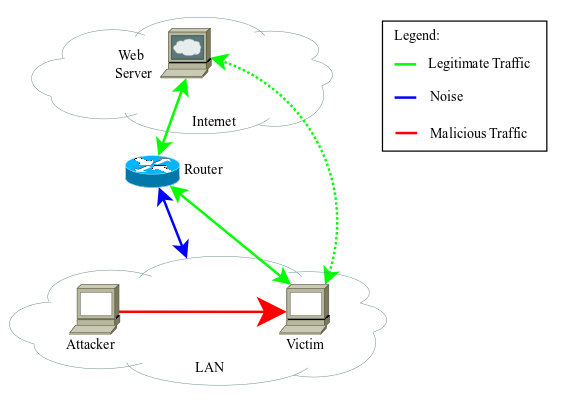
\includegraphics[height=5cm, width=7cm]{results/figures/fig09.png}
     \caption{Scenario to reproduce legitimate traffic, noise, flood and port scan.}
     \label{fig:fig1}
\end{figure}

Note that the set of network traffic is modeled as legitimate, noise and malicious traffic, where the victim performs legitimate activities, that can be characterized by web access. In many organizations this type of traffic is predominant, since most of corporate services are web-based, such as: web pages, customized web-based systems and cloud services. It is possible to characterize the traffic of a DHCP service as an example of noise associated with the transport layer. For malicious traffic, three types of networks attacks are evaluated: synflood, fraggle and port scan. These attacks are reproduced using well-known security tools, such as Nmap\footnote{http://nmap.org} to port scan, Metasploit\footnote{http://www.metasploit.com} to synflood and Hping\footnote{http://hping.org} to lead the fraggle attack.

A network traffic log is commonly formed by timestamp, protocol, source IP address, source port, destination IP address, destination port and additional information, according to the type of transport protocol used. The following TCP traffic log is presented in order to exemplify the collected data:
\newline
\newline
\texttt{\justify21:00:34.099289 IP 192.168.1.102.34712 > 200.221.2.45.80: Flags [S], seq 2424058224, win 14600, options [mss 1460, sackOK,TS val 244136 ecr 0,nop,wscale 7], length 0}
\newline

and the following to exemplify UDP traffic log: 
\newline
\newline
\texttt{\justify21:24:42.484858 IP 192.168.1.102.68 > 192.168.1.1.67: BOOTP/DHCP, Request from 00:26:9e:b7:82:be, length 300}
\newline 

In the proposed framework, the goal is to detect the anomalies only taking into account the traffic profile, i.e., specific information such as origin IP or day and time of the attack are not considered. Therefore, from the entire log information, we just consider the timestamp (for sequencing), port type and port number.

\subsection{Modeling Data}
\label{sec:ModelingData}

By modeling the dataset as a signal superposition, the network traffic (\textbf{X}) can be characterized as a mixture of three components: legitimate traffic (\textbf{U}), noise (\textbf{N}) and malicious traffic (\textbf{A}), according to the following expression:

\begin{equation}\label{eq:eq01}
\boldsymbol{X}^{(q)} = \boldsymbol{U}^{(q)} + \boldsymbol{N}^{(q)} + \boldsymbol{A}^{(q)},
\end{equation}
where $q$ represents the $q$-th time frame, which is a time grouping of network traffic. The matrix $\boldsymbol{X}^{(q)} \in \mathbb{R}^{M \times N}$ consists of \emph{M} rows and \emph{N} columns. Each row represents a communication port (TCP port or UDP port), and each column represents time bins having a approtiate size, such as one minute. Each element $x_{m,n}^{(q)}$ stands for the number of times that the port $m$ appears at the $n$-th minute, at the $q$-th time frame.

The legitimate traffic $\boldsymbol{U}^{(q)}$ is characterized by the traffic from user's operations. When a user accesses a web page, for example, there is the corresponding TCP/IP traffic to request the page, as well as there is the traffic required to domain name resolution. Figure \ref{fig:fig3} depicts an example of the legitimate traffic obtained during experiments.

\begin{figure}[h!]
     \centering 
     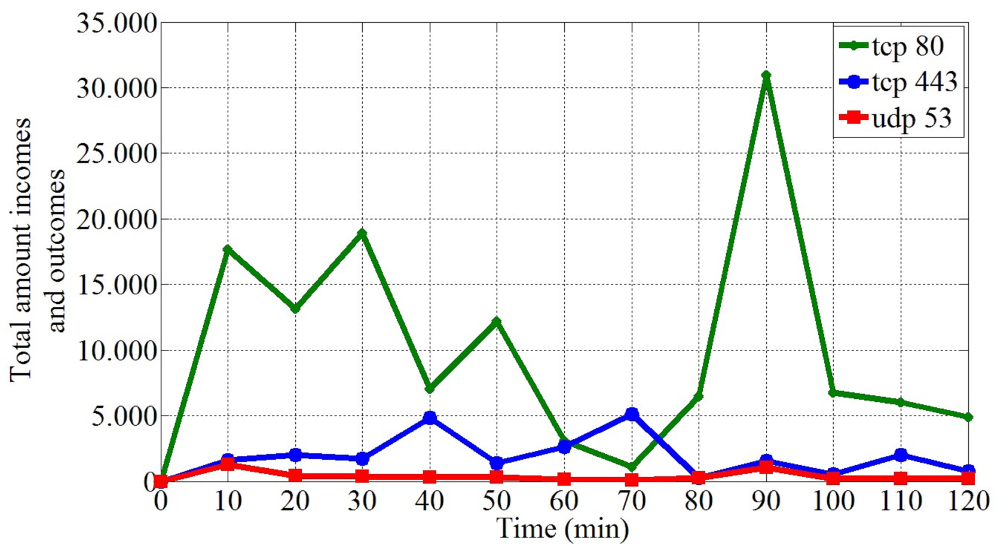
\includegraphics[height=4.5cm, width=9cm]{results/figures/fig03.png}
     \caption{Traffic from user's operations, that can be characterized by web access, traffic of well-known applications or network protocols.}
     \label{fig:fig3}
\end{figure}

The traffic that is not associated with user's operations and with malicious traffic is modeled as noise $\boldsymbol{N}^{(q)}$. The automatic acquisition service of logical IP network address (DHCP) is an example of noise. Independently of any user operation, the machine receives an IP address, since it is configured to perform a DHCP address request. Figure \ref{fig:fig4} depicts an example of noise in a network traffic, represented by traffic to ports 67 and 68.

\begin{figure}[h!]
     \centering 
     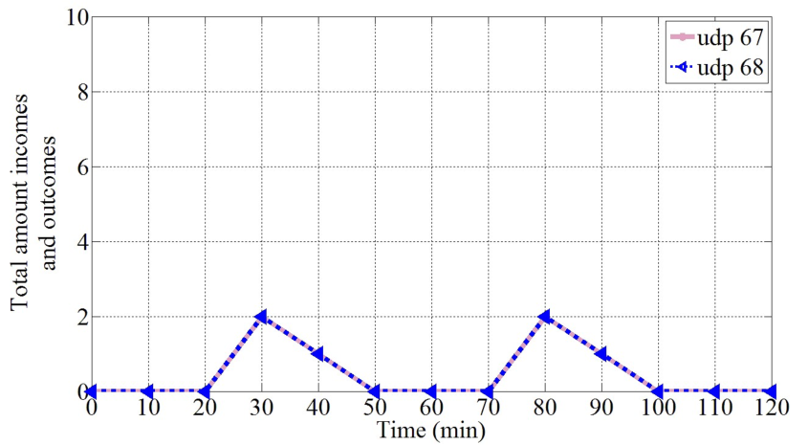
\includegraphics[height=4.5cm, width=9cm]{results/figures/fig04.png}
     \caption{Network traffic of user independent operations for network management.}
     \label{fig:fig4}
\end{figure}

The traffic coming from a malicious activity, such as a synflood or fraggle attack, is represented by the matrix $\boldsymbol{A}^{(q)}$. For this work we only consider the traffic from port scanning and flood attacks.

We define that if the obtained $\#\boldsymbol{A}^{(q)} ≠ 0$, then there is malicious traffic in the evaluated time frame $q$, on the other hand, if the $\#\boldsymbol{A}^{(q)} = 0$, then there is no malicious traffic. This paper shows how to detect the $\#\boldsymbol{A}^{(q)}$, given only the matrix $\boldsymbol{X}^{(q)}$, in order to identify malicious network traffic.

\subsection{Synflood, Fraggle and Port scan}
\label{sec:SynfloodFraggleandPortscan}

The network attacks evaluated by this work are: synflood, fraggle and port scan. The first two attacks can be qualified as flood or denial of service (DoS) attacks, while the last one can be qualified as probe or port scanning attack. DoS attempts to block access to system or network resources, it is implemented by either forcing targets to be unavailable through the exploiting of system vulnerabilities, or consuming resources through large amount of network traffic, characterizing flood attacks. Probe attacks scan the networks to to collect information about host, such as IP addresses, ports and services.


With respect to the synflood attacks, the attacker sends a large quantity and concurrent successive SYN requests to a target, in order to consume resources and cause a DoS. Figure \ref{fig:fig5} depicts an example of a synflood attack carried out in a real computer network. In an interval of ten minutes, more than 210,000 packets are sent as a synflood attack. This network traffic behavior can be considered an abnormal behavior of network traffic, especially since it is concentrated in a short period of time and presents similar outstanding traffic during the time under attack.

\begin{figure}[h!]
     \centering 
     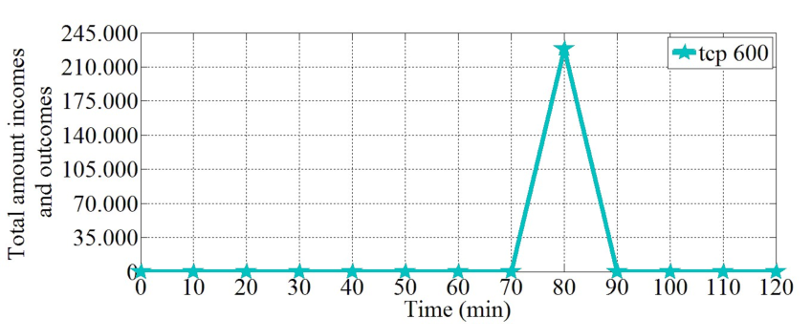
\includegraphics[height=4.5cm, width=9cm]{results/figures/fig05.png}
     \caption{A large quantity of SYN requests to a target, in order to cause a DoS.}
     \label{fig:fig5}
\end{figure}

With respect to the fraggle attack, large packets with UDP echo segments are sent to the broadcast address of a network. Every packet is modified to have the source address of the victim, in order to implement the source address spoofing technique. Therefore, each host receives a huge amount of requests UDP echo and all of them replies to the IP address of the victim, causing a packet flooding aiming a DoS. This attack can affect the entire network, since all hosts receive several requests UDP echo and respond with the ICMP protocol, therefore each host acts as an amplifier of the attack. This last part of the fraggle attack is not taken into account in this work, because the victim receives ICMP (network layer) packets originated from the hosts that are attacked with flooding packet UDP echo. Figure \ref{fig:fig6} depicts an example of the fraggle attack in a real computer network. 

\begin{figure}[h!]
     \centering 
     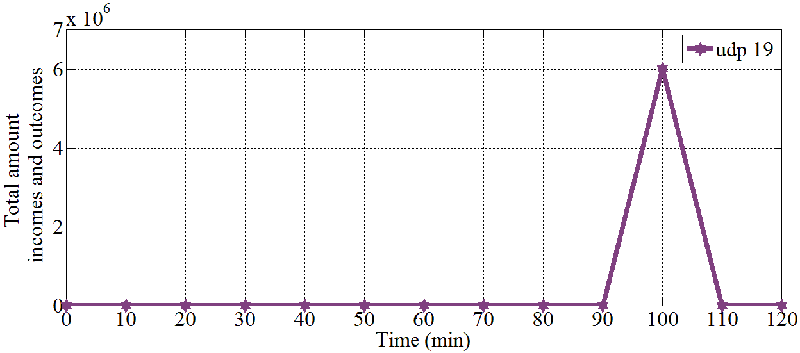
\includegraphics[height=4.5cm, width=9cm]{results/figures/fig06.png}
     \caption{Large amount of “UDP echo” requests and replies, causing packet flooding.}
     \label{fig:fig6}
\end{figure}

More than 6,000,000 malicious packets can be counted in an interval of ten minutes, which can be considered an abnormal network traffic, especially due to the concentrated traffic in a short period of time and due to the similarity of the outstanding traffic.

Port scan is the attempt to establish a connection to TCP and UDP ports to identify what services are running or are in the listening state. There are several available port scanning techniques, including: TCP SYN scan, TCP ACK scan and UDP scan. This work evaluates the use of TCP SYN scan and UDP scan. 

In TCP SYN scan, a SYN packet is sent to the destination and two types of responses may occur: SYN/ACK or RST/ACK. In the first case, the destination port is in the listening state, in the second case, the destination port is not listening. At the end of each port scanning, a RST/ACK packet is sent by the system that is performing the port scan. Therefore, a full connection or a complete three-way handshake is never established, which makes the detection of the attack sender more difficult, and requires approaches able to identify probe attacks without connection stablishment. The UDP scan technique sends UDP packets to the destination port, and if it responds with a \emph{ICMP port unreachable} message, then it indicates that the scanned port is closed. On the other hand, if a message is not received, then the port is considered as open.

\begin{figure}[h!]
     \centering 
     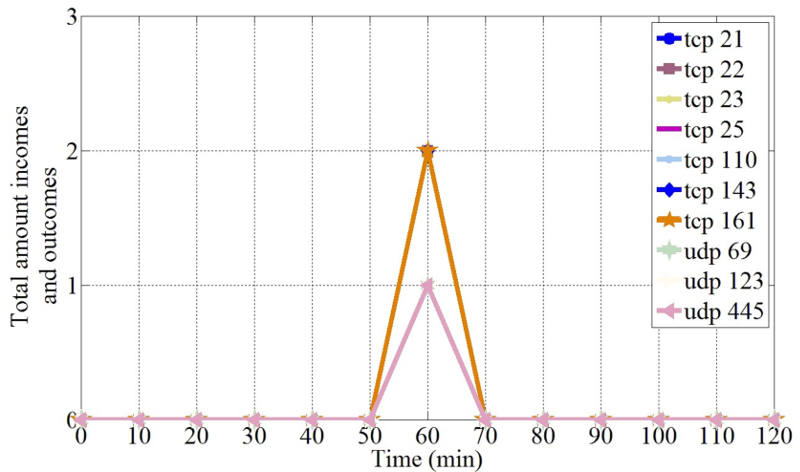
\includegraphics[height=5cm, width=9cm]{results/figures/fig07.png}
     \caption{Connection attempts in order to identify active ports.}
     \label{fig:fig7}
\end{figure}

Figure \ref{fig:fig7} depicts an example of the port scan attack in a real computer network. Note that the traffic is composed of two packets for each TCP port and one UDP packet to each port. The incoming and outgoing packets analysis, for each port, shows the high correlation and similarity of TCP and UDP traffic during the simulated port scan attack.

\subsection{The DARPA Dataset}
\label{sec:DarpaDataset}

The DARPA 1998 dataset\footnote{https://www.ll.mit.edu/ideval/data/} includes 7 weeks of sniffed traffic saved into raw TCPDUMP packet data, from inside and outside origins, with labeled attacks. The attacks in this dataset
can be grouped into: denial-of-service (DoS); remote to local (R2L), which is characterized by unauthorized access from a
remote machine; user to root (U2R), which is characterized by unauthorized access to local
super-user privileges; and probe attack. Since the proposed approach focus on flood and probe attack, we analyze the attacks that present behaviors similar to flood or probe attack. We observe that the most cases of DoS focus on exploit system vulnerabilities instead of on flooding attack. One example is the occurrence of a neptune attack which sends 20 only SYN packets, what is a behavior that differs of the expected flood attack behavior. Therefore, we select the cases that simulates several network traffic or numerous connection requests, also known as flooding attack \cite{ahmed2016survey,osanaiye2016distributed}, and the cases that scan ports sending just a few packets. From the simulated probe attacks, we select the cases that rely on TCP or UDP connections.

The data modeling follows the method described by the Subsection \ref{sec:ModelingData}, with time frames of 20 minutes, packet counting aggregation by minute and considering the traffic to the following ports: 20, 21, 22, 23, 25, 79, 80, 88, 107, 109, 110, 113, 115, 143, 161, 389, 443.


\section{Proposed Framework for Detection and Identification of Network Attacks}
\label{sec:prop_getv}

This section describes the proposed technique to detect synflood, fraggle and port scan, according to Figure \ref{fig:fig80}, which represents the overview of the proposed framework for detection and identification of network attacks. In Subsection \ref{sec:prop_LargestEigenvaluebyTimeFrames} we present the steps for extraction of the largest eigenvelue for each $q$-th time frame. Next, in Subsection \ref{sec:prop_MOSSchemes}, we show how to apply the eiganvalues on the MOS scheme in order to detect the attack. In Subsection \ref{sec:prop_EigenvalueAnalysis}, we present the eigenvalue analysis to identify the time frames detected as under attack, and the Subsection \ref{sec:prop_EigenSimilarityAnalysis} describes the similarity analysis evaluated for detailed attack identification.

\begin{figure}[h!]
	\centering
     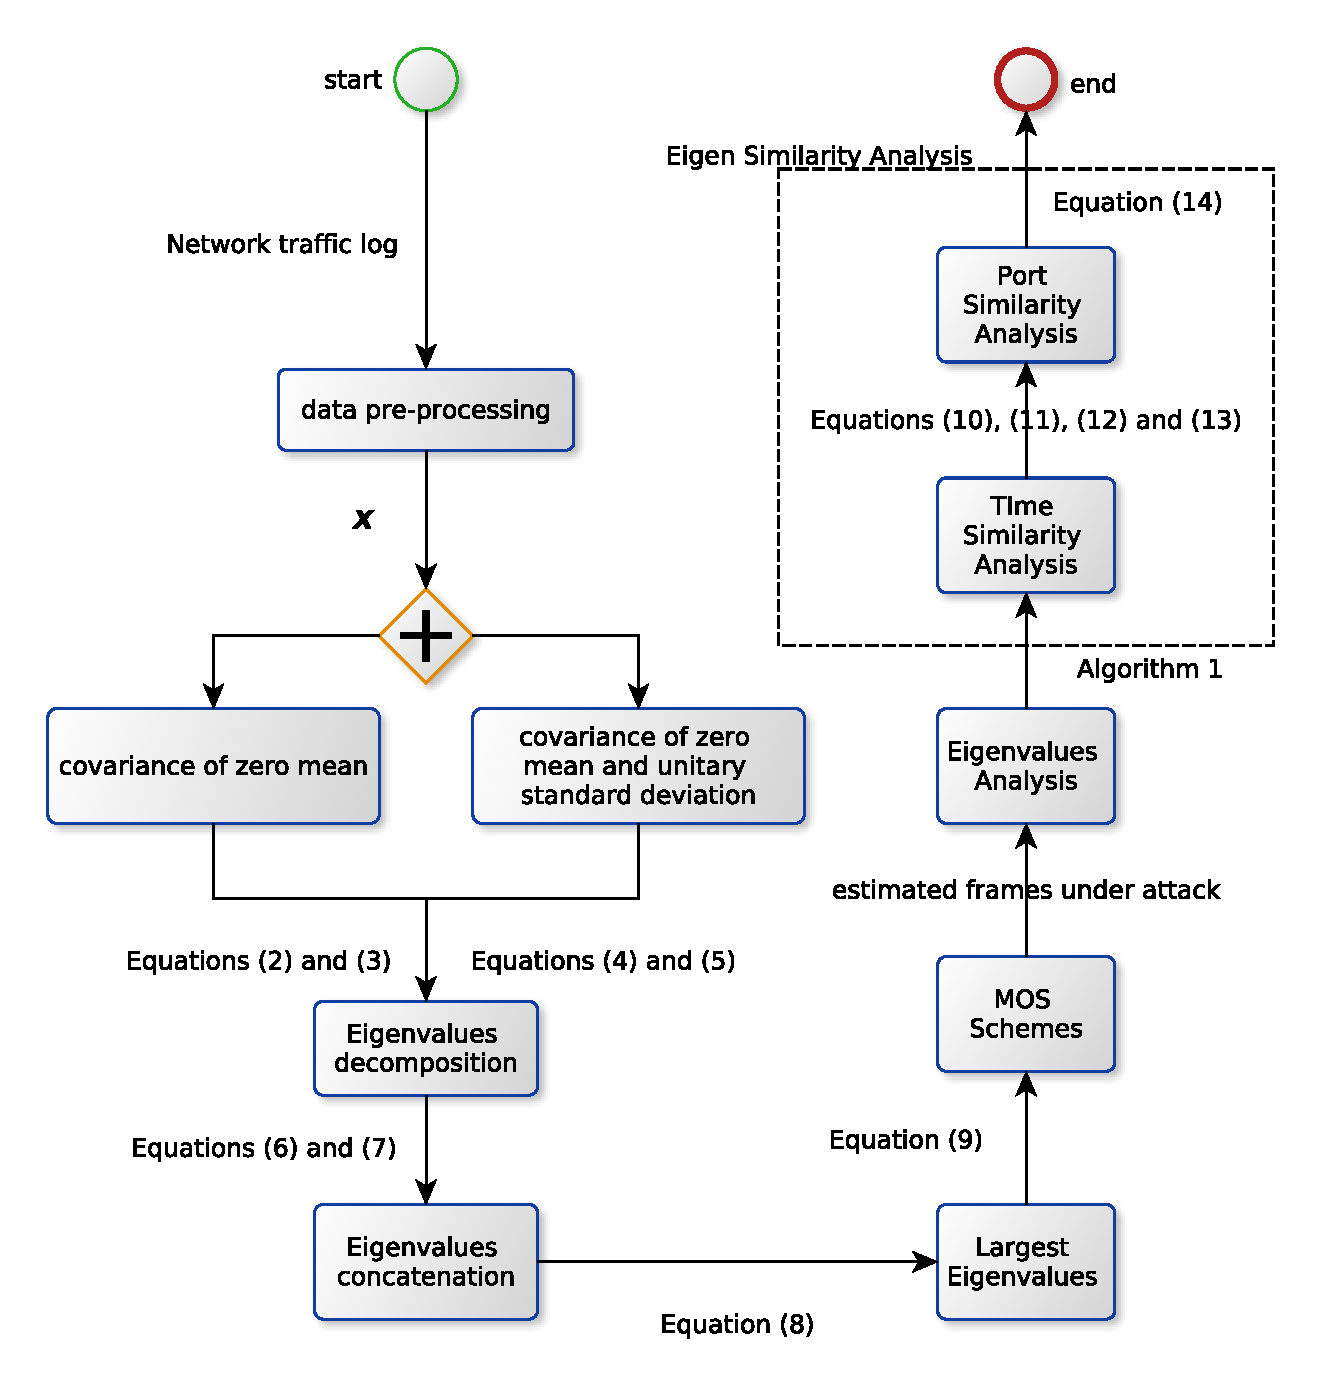
\includegraphics[height=11cm, width=9cm]{results/figures/mos_eigen_similarity.eps}
     \caption{Overview of The Framework for Detection and Identification of Network Attacks.}
     \label{fig:fig80}
\end{figure}

\subsection{Largest Eigenvalue by Time Frames}
\label{sec:prop_LargestEigenvaluebyTimeFrames}

The proposed attack detection algorithm starts by the data pre-processing of a network traffic log containing IP, ports and timestamp of senders and receivers. During this step, the desired information is extracted in order to classify and count packets according to the origin and destination ports, and subsequently this information is grouped by minutes and by time frames.

With the data grouped into $Q$ time frames, the framework considers the time variations of the matrix $\boldsymbol{X}^{(q)} \in \mathbb{R}^{M\times{N}}$, with $q = 1, \ldots, Q$, in order to detect the attack. 

According to flood and port scan attacks' behavior, flood attacks and port scan attacks can be characterized as covariance aware attack \citep{jin2004covariance} and correlation aware attack \citep{lakhina2005mining}, respectively. These characteristics are substantiated by the results obtained through the analysis based on sample covariation of zero mean variables and on covariance of zero mean and unitary standard deviation variables, described in Section \ref{sec:experimentalresults}, which shows that the main components of flood attacks are dominated by the variables with more variance and that the traffic associated with port scan attack does not generate many logs, however, it presents high covariance of zero mean and unitary standard deviation variables.

Therefore, to detect flood attacks, it is necessary to calculate the sample covariance matrix $\boldsymbol{\hat{R}}_{yy}^{(q)}$ of the zero mean samples given by

\begin{equation}\label{eq:eq02}
\boldsymbol{y}_{m}^{(q)} = \boldsymbol{x}_{m}^{(q)} - \bar{\boldsymbol{x}}_{m}^{(q)}.
\end{equation}

The set of obtained vectors $\boldsymbol{y}_{m}^{(q)}$ composes the zero mean matrix $\boldsymbol{Y}^{(q)}$, then the sample covariance matrix $\boldsymbol{\hat{R}}_{yy}^{(q)}$ can be calculated as follows

\begin{equation}\label{eq:eq03}
\boldsymbol{\hat{R}}_{yy}^{(q)} = \frac{1}{N}\boldsymbol{Y}^{(q)}\boldsymbol{Y}^{(q)^{\rm T}}.
\end{equation}

For the detection of the port scan attack, the main components are not dominated by the variables with large variance. Moreover, the portscan traffic presents a highly correlated network traffic. In order to exploit such structure, we compute the sample covariance $\boldsymbol{\hat{R}}_{zz}^{(q)}$ whose variables have zero mean and unitary standard deviation as follows

\begin{equation}\label{eq:eq04}
\boldsymbol{z}_{m}^{(q)} = \frac{\boldsymbol{x}_{m}^{(q)} - \bar{\boldsymbol{x}}_{m}^{(q)}}{\boldsymbol{\sigma}_{m}^{(q)}}.
\end{equation}

The set of vectors $\boldsymbol{z}_{m}^{(q)}$ composes the matrix $\boldsymbol{Z}^{(q)}$, then the sample covariance matrix $\boldsymbol{\hat{R}}_{zz}^{(q)}$ can be calculated via 

\begin{equation}\label{eq:eq05}
\boldsymbol{\hat{R}}_{zz}^{(q)} = \frac{1}{N}\boldsymbol{Z}^{(q)}\boldsymbol{Z}^{(q)^{\rm T}}.
\end{equation}

Once the $\boldsymbol{\hat{R}}_{yy}^{(q)}$ and $\boldsymbol{\hat{R}}_{zz}^{(q)}$ have been obtained for flood and port scan attack detection, respectively, and since the next steps are the same for both sample covariance matrices, we refer to $\boldsymbol{\hat{R}}_{yy}$ and $\boldsymbol{\hat{R}}_{zz}$ as a matrix $\boldsymbol{C}$. Therefore, the following step of the algorithm is the eigenvalue decomposition (EVD), calculated according to (\ref{eq:eq06}), in order to obtain the vector of eigenvalues $\boldsymbol{e}^{(q)}$ associated with each matrix, according to (\ref{eq:eq060}).

\begin{equation}\label{eq:eq06}
\boldsymbol{C}^{(q)} = \boldsymbol{V}^{(q)}\boldsymbol{\Lambda}^{(q)}\boldsymbol{V}^{(q)^{\rm T}},
\end{equation}

\begin{equation}\label{eq:eq060}
\boldsymbol{e}^{(q)} = \rm diag(\boldsymbol{\Lambda}^{(q)}),
\end{equation}

where the operator diag$(\cdot)$ extracts the main diagonal of a matrix.

The eigenvalues should be sorted in descending order, i.e., $\lambda_{1}^{(q)} > \lambda_{2}^{(q)} > \lambda_{3}^{(q)} > ... > \lambda_{m}^{(q)}$. Therefore, the largest eigenvalue of the $q$-th time frame evaluated for the attack detect is given by $\lambda_{1}^{(q)}$.

The concatenation of the eigenvalues vector $\boldsymbol{e}^{(q)}$ for $q = 1, \ldots, Q$ is represented by

\begin{equation}\label{eq:eq07}
\boldsymbol{E} =
\begin{bmatrix}
  \lambda_1^{(1)} & \lambda_1^{(2)} & \lambda_1^{(3)} & \cdots & \lambda_1^{(Q)} \\
  \lambda_2^{(1)} & \lambda_2^{(2)} & \lambda_2^{(3)} & \cdots & \lambda_2^{(Q)} \\
  \lambda_3^{(1)} & \lambda_3^{(2)} & \lambda_3^{(3)} & \cdots & \lambda_3^{(Q)} \\
  \vdots & \vdots & \ddots & \vdots  \\
  \lambda_m^{(1)} & \lambda_m^{(2)} & \lambda_m^{(3)} & \cdots & \lambda_m^{(Q)} \\
\end{bmatrix}.
\end{equation}

Note that since $\lambda_1^{(q)} > \lambda_2^{(q)} > \lambda_3^{(q)} > \cdots > \lambda_{m-1}^{(q)} > \lambda_m^{(q)}$, then the first line of the matrix $\boldsymbol{E}$ contains the largest eigenvalues of each $q$-th time frame, which is the Greatest Eigenvalue Time
Vector (GETV) \cite{tenorio2013greatest}, denoted as 

\begin{equation}\label{eq:eq08}
\boldsymbol{e}_{\rm max} = \boldsymbol{E}\{:,1\} = [ \lambda_1^{(1)}, \lambda_1^{(2)} ... \lambda_1^{(Q)}]
\end{equation}

\subsection{MOS Schemes}
\label{sec:prop_MOSSchemes}

Traditionally the MOS schemes are applied for the eigenvalues of the vector $\boldsymbol{e}^{(q)}$. However, the goal here is to detect the variations of the eigenvalues for different values of $q$. Therefore, instead of using a certain $q$, the proposed approach applies MOS schemes for a vector of the largest eigenvalues of each $q$-th time frame, in order to identify variations and estimate the model order $\hat{d}$, which is the estimated number of time frames under attack. Therefore, $\boldsymbol{e}_{\rm max}$ is sorted in descending order, producing $\sim\boldsymbol{e}_{\rm max}$, that is used as input parameter for MOS schemes, according to $\hat{d} = \rm{MOS}(\sim\boldsymbol{e}_{\rm max})$. Note that some MOS schemes may also require the number of minutes that compose a time frame, as $\hat{d} = \rm{MOS}(\boldsymbol{e}_{\rm max},\emph{Q})$. For more information about MOS, we refer to \ref{sec:mos}.

In our previous work \cite{tenorio2013greatest}, the accuracy of AIC, MDL, EDC, RADOI, EFT and SURE schemes are evaluated for synflood and port scan attack detection, showing that EDC and EFT are effective for detecting this kind of attacks. The present work extends that evaluation to also analyse the effectiveness of the listed MOS schemes for fraggle attack detection, as shown in Section \ref{sec:experimentalresults}.

\subsection{Eigenvalue Analysis}
\label{sec:prop_EigenvalueAnalysis}

After applying the MOS schemes to the vector $\sim\boldsymbol{e}_{\rm max}$, we obtain the estimate of the $\#\boldsymbol{A}$. For instance, in the case of fraggle, synflood and portscan, if $\hat{d} = 1$, , then $\#\boldsymbol{A} = 1$, which means that during the during the $Q$ time frames one attack is present. However, if $\hat{d} = 0$, then $\#\boldsymbol{A} = 0$, and this means that none of these attacks are present. Note that $\hat{d}$ can be greater than 1, indicating the presence of more than one attack.

In Subsection \ref{sec:prop_MOSSchemes}, we obtained only if $\hat{d} = 1$ or $\hat{d} = 0$. However, if $\hat{d} = 1$, the MOS schemes do not provide any information about the $q$-th time frame under attack. The identification of the $q$-th time frame under attack can be carried out through a eigenvalues analysis.

The largest eigenvalue analysis for estimating the $q$-th time frames that are under attack can be expressed according to Algorithm \ref{alg:alg01}, where $\rm{\boldsymbol{\hat{q}}}_{\rm max} \in \mathbb{R}^{\hat{d}}$ denotes a vector of the $q$-th time frames under attack, which is the $q$-th indexes corresponding to the $\hat{d}$ largest eigenvalues of $\boldsymbol{e}_{\rm max}$. Algorithm \ref{alg:alg01} initially identifies the largest value of $\boldsymbol{e}_{\rm max}$, according to Line 2 of Algorithm \ref{alg:alg01}, and its correspondent index, according to Lines 4 and 5 of Algorithm \ref{alg:alg01}. Subsequently, the largest value is removed of $\boldsymbol{e}_{\rm max}$, according to Line 8 of Algorithm \ref{alg:alg01}, and a new iteration is performed until $\boldsymbol{e}_{\rm max} = \{\}$.

\begin{algorithm}[h!]
	\caption{Detection of Time Frames Under Attack}
  	\label{alg:alg01}
	\begin{algorithmic}[1]
		\show\LOOP
	    \ALOOP {$f = 1$ until $f == \hat{d}$} 
	    	    \STATE $q_{\rm value} = \argmax\limits_{\lambda}  \hspace{1 mm} \boldsymbol{e}_{\rm max}$
    	    	    \ALOOP {$i = 1$ until $i == Q$} 
				\IF {$\boldsymbol{e}_{\rm max}^{(i)} == q_{\rm value}$}
				    \STATE $\boldsymbol{\hat{q}}_{\rm max}^{(f)} = i$
				\ENDIF
        		\ENDALOOP
	    		\STATE $\boldsymbol{e}_{\rm max} \rightarrow \boldsymbol{\hat{q}}_{\rm max}^{(f)}$
    		\ENDALOOP
	\end{algorithmic}
\end{algorithm}

After the estimation of the $\rm{\boldsymbol{\hat{q}}}_{\rm max}$ time frames under attack, it is necessary to obtain more details of the detected attacks, such as the $n$-th minutes when the attacks happened and the $m$-th network ports that were attacked. To deal with this problem, the adoption of a similarity analysis between legitimate traffic and the traffic of time frames estimated as under attack is evaluated, analysing the effectiveness of cosine similarity to highlight abnormalies inserted by network traffic attacks. 

\subsection{Eigen Similarity Analysis}
\label{sec:prop_EigenSimilarityAnalysis}

Cosine similarity calculates the cosine of the angle between two vectors, which represents the similarity of values between the selected vectors. Therefore, cosine similarity can be used to evaluate the variation of the most significant eigenvectors of $\boldsymbol{V}^{(q)}$ against the the most significant eigenvectors of time frame detected as under attack, to analyse similarity changes into the most significant eigenvectors caused by the insertion of anomalous traffic \cite{Lee2013}. 

This subsection describes the proposed eigen similarity analysis for detailed attack identification, in complement to the attack estimation carried out through MOS schemes and eigenvalue analysis. In Subsection \ref{sec:prop_TimeSimilarityAnalysis} we present the eigen similarity analysis for identification of time under attack. Next, in Subsection \ref{sec:prop_PortSimilarityAnalysis}, we show how to apply the eigen similarity analysis in order to identify network ports under attack.

\subsubsection{Time Similarity Analysis}
\label{sec:prop_TimeSimilarityAnalysis}

For eigen similarity analyis, we evaluate the cosine similarity in order to identify lacks of similarity between legitimate and malicious traffic, as follows

\begin{equation}\label{eq:eq11}
s_n = \frac{\abs{\boldsymbol{v}^{(q)} \cdot \boldsymbol{v}_{(n)}}}{\norm{\boldsymbol{v}^{(q)}}\norm{\boldsymbol{v}_{(n)}}},
\end{equation}
where $s_n$ denotes the absolute similarity degree of the $n$-th minute, $\boldsymbol{v}^{(q)}$ is the most significant eigenvectors of a selected set of minutes without network attack, and $\boldsymbol{v}_{(n)}$ is the most significant eigenvectors obtained after append the target $n$-th minute of traffic to be performed the flood and port scan attack identification.

The most significant eigenvector $\boldsymbol{v}^{(q)}$, of a time frame $q$ without attack, can be derivated from (\ref{eq:eq06}) and selected according to the eigenvector of the largest eigenvalue $\lambda_1^{(q)}$, which is the principal component of the evaluated matrix. The same calculation shall be performed in order to obtain the target eigenvectors $\boldsymbol{v}_{(n)}$, calculated from a time frame without attack plus minutes of a time frame estimated as under attack, to evaluate the occurrence of network attacks. 

The reference eigenvectors $\boldsymbol{v}^{(q)}$ is calculated from the traffic whithout attack, from a time frame $q$ composed of $Q$ minutes of legitimate network traffic. For the detailed attack identification, each $\boldsymbol{x}^{(\hat{q})}_{(n)}$ vector of each $n$-th minutes of the estimated $\rm{\boldsymbol{\hat{q}}}_{\rm max}$ time frames shall be individually appended into $\boldsymbol{X}^{(q)}$, as represented by

\begin{equation}\label{eq:eq12}
\boldsymbol{X}_{n} = \{\boldsymbol{X}^{(q)} | \boldsymbol{x}^{(\hat{q})}_{(n)}\}.
\end{equation}

The resultant $\boldsymbol{X}_{(n)}$ is necessary to obtain $\boldsymbol{v}_{(n)}$, through (\ref{eq:eq06}), for calculating the similarity degree $s_n$, ranging from 0 to 1, for each $n$-th minute. The $s_n$ denotes the absolute similarity degree of the $n$-th minute in comparison to a well-known traffic without attack, detected through MOS schemes and eigenvalue analysis.

The incremental approach for similarity analysis is based on the incremental appending of network traffic into $\boldsymbol{X}^{(q)}$, where the first evaluation is based on (\ref{eq:eq12}) and the subsequent evaluations is based on (\ref{eq:eq13}), incrementally appending each $n$-th minute until $n=N$.

\begin{equation}\label{eq:eq13}
\boldsymbol{X}_{n} = \{\boldsymbol{X}_{n} | \boldsymbol{x}^{(\hat{q})}_{(n)}\},
\end{equation}

Figure \ref{fig:fig8} ilustrates the network traffic selection for the incremental approach of eigen similarity analysis, where the $\boldsymbol{X}^{(1)}$ is chosen as reference for similarity analysis of the $m$-th minutes of the time frame $q=3$, where one network attack was previously detected. 

\begin{figure}[h!]
     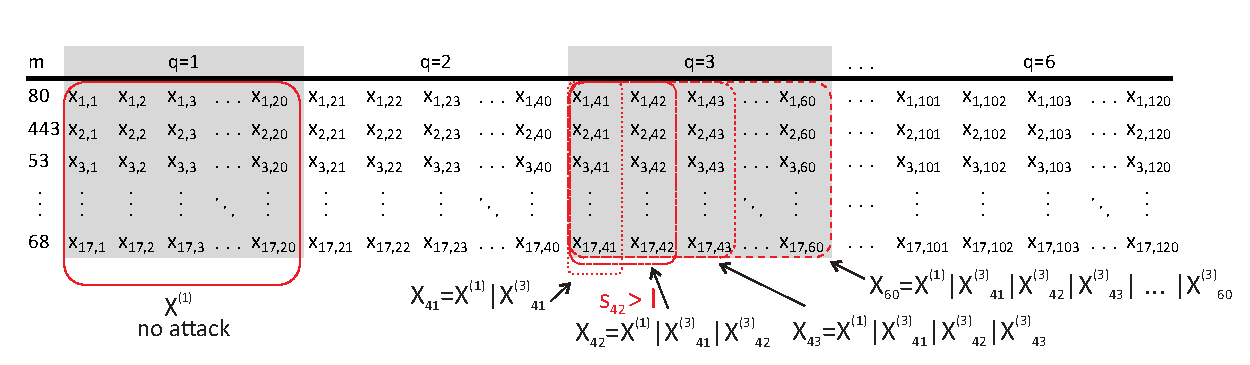
\includegraphics[height=4cm, width=12.4cm]{results/figures/incremental.eps}
     \caption{Traffic selection for incremental approach.}
     \label{fig:fig8}
\end{figure}

The eigen similarity analysis starts at $\boldsymbol{x}^{(3)}_{(41)}$ and is incrementally performed until $\boldsymbol{x}^{(\hat{3})}_{(60)}$, in order to calculate the $s_n$. We assume that $s_n < l$ means an attack identification, according the anomaly on similiarity of $s_n$ to a defined limiar $l$. Therefore, after obtaining the most significant eigenvector $\boldsymbol{v}^{(q)}$ and the target eigenvectors $\boldsymbol{v}_{(n)}$ for eigen similarity analyis, the $s_n$ is calculated according to~(\ref{eq:eq11}).

If $s_n = 1$, then the two eigenvectors are completely similar and no anomaly is detected. Smaller values of $s_n$ mean less similarity and can indicate an anomaly, according to a defined 
threshold $l$, assuming that if $s_n < l$, then a network attack is identified during the $n$-th minute. Therefore, the $s_n$ of each $n$-th minute shall be compared with the threshold $l$ to evaluate if a attack was identified, according to

\begin{equation}\label{eq:eq14}
  \boldsymbol{\hat{n}_{(n)}}=\left\{
  \begin{array}{@{}ll@{}}
    1, & \text{if}\ s_n < l \\
    0, & \text{otherwise}
  \end{array}\right.
\end{equation}
where $\boldsymbol{\hat{n}}_{(n)}$ denotes a vector of $n$-th minutes detected as under attack.

The eigen similarity analysis can also be applied in an individual fashion, where each $n$-th minute must be individually appended into $\boldsymbol{X}^{(q)}$, as shown by Figure \ref{fig:fig9}.

\begin{figure}[h!]
     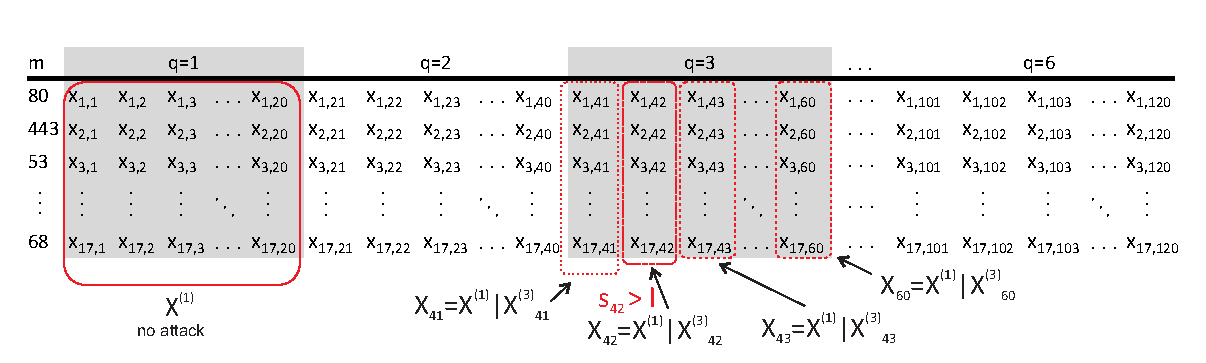
\includegraphics[height=4cm, width=12.4cm]{results/figures/individualized.eps}
     \caption{Traffic selection for individual approach.}
     \label{fig:fig9}
\end{figure}

The incremental and the individual approaches can be combined to obtain the incremental individualized approach, where each minute is incrementally appended into the selected $\boldsymbol{X}^{(q)}$ for obtaining $\boldsymbol{v}_{(n)}$ to similarity analysis of the $n$-th minute, until detect the first $n$-th minute under attack. Subsequently, $\boldsymbol{X}_n$ becomes the new reference of traffic without network attack and each subsequent minute must have its similarity individually evaluated, as shown in Figure \ref{fig:fig2}.

\begin{figure}[h!]
     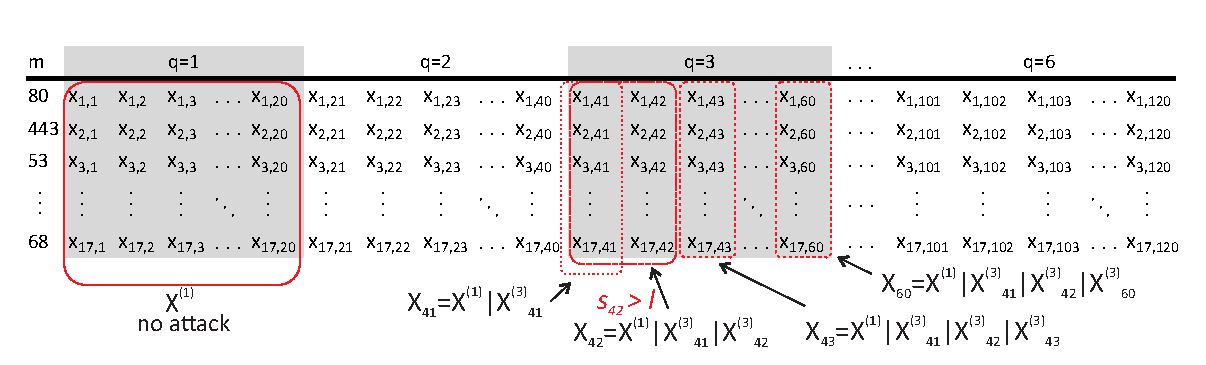
\includegraphics[height=4cm, width=12.4cm]{results/figures/incremental_individualized.eps}
     \caption{Traffic selection for incremental individualized approach.}
     \label{fig:fig2}
\end{figure}

This approach of incremental similarity analysis followed by individual analysis after an attack detection allows to identify the attack period, highlighting the first and last time under attack. This identification is possible due to the variation of the most significant eigenvectors, which becomes more significant when compared a traffic under attack against a traffic with no attack, according to results which are discussed in Section \ref{sec:experimentalresults}.

\subsubsection{Port Similarity Analysis}
\label{sec:prop_PortSimilarityAnalysis}

Given $\boldsymbol{\hat{n}}$, which is the set of $n$-th minutes under attack, it is still necessary to obtain more details about the identified network attack, such as the network ports that are attacked during each $n$-th minute identified as under attack. Hence, it is also applied the cosine similarity analysis to identify variation of the most significant eigenvectors, caused by the insertion of anomalous network traffic by a selected $m$-th port during a $n$-th minute. 

For detection of ports under attack, the $\boldsymbol{v}^{(q)}$ last most significant eigenvectors without attack shall be used as reference for similarity analysis against the $\boldsymbol{v}_{(n)}$ identified as under attack, individually evaluating the cosine similarity of each $m$-th port of all $\boldsymbol{\hat{n}}$ minutes.

Therefore, $\boldsymbol{v}^{(q)}$ should be calculated from the last $\boldsymbol{X}^{(q)}$ time frame without attack, and $\boldsymbol{v}_{(m,\hat{n})}$ should be calculated from the same traffic appened of all $n$-th minutes until the identified minute under attack, denoted as $\boldsymbol{X}_n$. 

For similarity analyis, each $m$-th port of the last $n$-th minute of $\boldsymbol{X}_n$, denoted as $x_{(m,n)}$, shall be individually replaced by the traffic of the evaluated $m$-th port of the $\hat{n}$-th minute under attack, denoted as $x^{(\hat{q})}_{(m,\hat{n})}$, in order to identify significant variation on similarity caused by the traffic of the $m$-th port. 

This approach for detection of ports under attack via similarity analysis is given by

\begin{equation}\label{eq:eq15}
  \left\{
  \begin{array}{@{}ll@{}}
    x_{(m,n)} = x^{(\hat{q})}_{(m,\hat{n})} \\
    \\
    s_{m,\hat{n}} = \frac{\abs{\boldsymbol{v}^{(q)} \cdot \boldsymbol{v}_{(m,\hat{n})}}}{\norm{\boldsymbol{v}^{(q)}}\norm{\boldsymbol{v}_{(m,\hat{n})}}},
  \end{array}\right.
\end{equation}

where $x^{(\hat{q})}_{(m,\hat{n})}$ denotes the $m$-th port of the selected $n$-th minute identified as under attack and $x_{(m,n)}$ denotes the $m$-th port of the last $n$-th minute of $\boldsymbol{X}_n$, which is used to calculate the $\boldsymbol{v}_{(m,\hat{n})}$ most significant eigenvectors that contains the traffic of the $m$-th port of the $\hat{n}$-th minute identified as under attack.

Once $\boldsymbol{v}^{(q)}$ and $\boldsymbol{v}_{(m,\hat{n})}$ are obtained, then the $s_{m,\hat{n}}$ similarity degree can be calculated in order to identify if the traffic replacement highlights the adition of anomalous traffic by the evaluated $m$-th port during the $\hat{n}$-th minute previously identified as under attack. 

This procedure should be repeated for each $m$-th target port of $\boldsymbol{\hat{n}}$, in order to individually identify the network ports under attack during each $\hat{q}$-th time frame.

\section{Experiments and Results}
\label{sec:experimentalresults}

This section presents the performed experiments and the acquired results. First, in Section \ref{sec:AnalyzedScenario}, the simulated scenario adopted in the experiments is summarized. Then, Section \ref{sec:largesteigenvaluesanalysis} shows the results of the largest eigenvalue analysis by time frames for the simulated scenario. In Section \ref{sec:MOSSchemesEvaluation} are described the results of the evaluated MOS schemes for attack detection in the simulated dataset. Section \ref{sec:EigenvalueAnalysis} presents the results of the eigenvalue analysis for identification of time frames under attack, Section \ref{sec:EigenSimilarityAnalysis} shows the results of similarity analysis for detailed flood and port scan identification for the simulated scenario. Section \ref{sec:DarpaEvaluation} presents the results of the largest eigenvalue analysis, model order selection and the eigenvalue analysis for flood and probe attack detection in the DARPA 1998 dataset.

\subsection{Simulated Scenario}
\label{sec:AnalyzedScenario}

The experiment time is 120 minutes, separated into six time frames, with each time frame corresponding to twenty minutes. Therefore, as the time of each sampling period is one minute, then $N = 20$. For each time frame $q$, a traffic matrix $\boldsymbol{X}^{(q)} \in \mathbb{R}^{17 \times 20}$ was obtained, as well as a covariance $\boldsymbol{\hat{R}}_{yy}^{(q)} \in \mathbb{R}^{17 \times 17}$ (calculated via (\ref{eq:eq03})) and a sample covariance matrix $\boldsymbol{\hat{R}}_{zz}^{(q)} \in \mathbb{R}^{17x17}$, assuming that $q = 1, 2, 3, 4, 5$ and $6$. 

The simulation started at 21:00h, the first time frame was from 21:00h until 21:20h ($q = 1$), the second was from 21:20h until 21:40h ($q = 2$), the third was from 21:40h to 22:00h ($q = 3$), the fourth was from 22:00h until 22:20h ($q = 4$), the fifth was from 22:20h until 22:40h ($q = 5$), and finally, the sixth was from 22:40h until 23.00h ($q = 6$). During the simulation, the victim made legitimate access, and the attacker performed the following attacks: at 21:54h ($q = 3$) was performed a port scan, at the interval ranging from 22:10h to 22:20h ($q = 4$) a synflood attack was simulated, and at the interval from 22:30h to 22:40h ($q = 5$) a fraggle attack was performed.

\subsection{Largest Eigenvalues Analysis}
\label{sec:largesteigenvaluesanalysis}

For the evaluation of MOS Schemes accuracy for flood and port scan detection, the framework defines that it is necessary to obtain the largest eigenvalue of each time frame, through eigen decomposition from a covariance of zero mean variables or covariance matrix of zero mean and unitary standard deviation variables, calculated from the evaluated traffic, as described in Section \ref{sec:prop_getv}. Through eigenvalue analysis of traffic with flood or port scan attacks, it is possible to visualize a significant difference between the largest eigenvalues and the remain eigenvalues, which can indicate a relationship between an outlier and time frames under attack.

\begin{figure}[h!]
	\centering
     \includegraphics[height=6cm, width=8cm]{results/figures/eigenvalues_synflood.eps} 
     \caption{Eigenvalues of the sample covariance matrix (synflood).}
     \label{fig:fig10}
\end{figure}

Figure \ref{fig:fig10} depicts the eigenvalues calculated from sample covariance matrix of the network traffic used to evaluate the synflood attack identification. In Figure \ref{fig:fig10}, the largest eigenvalue related to the simulated synflood attack ($q = 4$) stands out significantly from the other eigenvalues.

Figure \ref{fig:fig11} illustrates the eigenvalues calculated from sample covariance matrix of the matrix used for fraggle attack detection. In Figure \ref{fig:fig10}, the largest eigenvalue related to the simulated synflood attack ($q = 5$) stands out significantly from the other eigenvalues, in accordance with the result shown in Figure \ref{fig:fig10} for the synflood attack analysis.

\begin{figure}[h!]
	\centering
     \includegraphics[height=6cm, width=8cm]{results/figures/eigenvalues_fraggle.eps}
     \caption{Eigenvalues of the sample covariance matrix (fraggle).}
     \label{fig:fig11}
\end{figure}

Figure \ref{fig:fig12} depicts the eigenvalues calculated from covariance matrix of zero mean and unitary standard deviation variables, of the network traffic matrix evaluated for port scan detection. 

\begin{figure}[h!]
	\centering
     \includegraphics[height=6cm, width=8cm]{results/figures/eigenvalues_portscan.eps}
     \caption{Eigenvalues of the covariance matrix of zero mean and unitary standard deviation (port scan).}
     \label{fig:fig12}
\end{figure}

As analyzed for the synflood and fraggle attacks, note that the largest eigenvalue, related to this attack ($q = 3$), stands out significantly from the others eigenvalues.

Table \ref{tab:tab3} presents the values of the largest eigenvalues of each time frame $q$-th for port scan, synflood and fraggle detection. 

\begin{table}[h!]
  \centering
  \footnotesize
  \caption{Largest Eigenvalue related to attacks detection}
  \label{tab:tab3}
  \begin{tabular}{ c c c c c }
	\toprule
	\multirow{3}{*}{\textbf{Time Frame} $q$} &\multicolumn{4}{c }{\textbf{Vectors GETV}}\\ 
			\hhline{~----}
		&\textbf{Detection of}	 &\textbf{Detection of}	 &\textbf{Detection of}	 &\textbf{Detection of}\\
		&\textbf{\emph{synflood/fraggle}}	 &\textbf{\emph{synflood}}	 &\textbf{\emph{fraggle}}	 &\textbf{\emph{port scan}}\\
	\midrule
	1 &1887545 &1887545 &1887545 &2,0734 \\
	2 &2341327 &2341327 &2341327 &2,1451 \\
	3 &3213867 &3213867 &3213867 &10,0718 \\
	4 &133238294 &133238294 &731229 &2,1620 \\
	5 &92384021611 &6367983 &92384021611 &2,4253 \\
	6 &708335 &708335 &708335 &1,7948 \\
    \bottomrule
  \end{tabular}
\end{table}

In Table \ref{tab:tab3}, note the significant variation of the eigenvalues associated with attacks, in comparison to the others. At $q = 4$, where the synflood attack occurred, the maximum eigenvalue obtained is approximately 21 times larger than the second one. At $q = 5$, where the fraggle attack occurred, the maximum eigenvalue obtained is about 29,000 times larger than the second one. At $q = 3$, where the port scan attack occurred, the maximum eigenvalue obtained is approximately 4 times larger than the second one. In the last case, for port scan attack detection, although the largest eigenvalue presented no too large variance to the second one, if compared to synflood or fraggle attacks, it clearly deviates from the remaining largest eigenvalues.

These results highlight that all $q$-th time frames where a network attack was simulated, present high significant variance between the largest eigenvalue and the remaining eigenvalues, obtained from sample covariance matrix, for flood detection, or from covariance matrix of zero mean and unitary standard deviation variables, for port scan detection. Therefore, we propose to apply the vector of the largest eigenvalues to MOS schemes in order to evaluate their accuracy for identification of time frames under attack, motivated by the fact that it is relevant to apply MOS schemes to automate the attack detection process, taking into account the characteristics of the evaluated eigenvalues.

\subsection{MOS Schemes Evaluation}
\label{sec:MOSSchemesEvaluation}

In \cite{tenorio2013greatest}, we evaluate the accuracy of AIC, MDL, EDC, RADOI, EFT and SURE MOS schemes \cite{da2009comparison,tenorio2013greatest} for synflood and port scan attack detection. In this work we extend that evaluation for fraggle attack detection, applying the same schemes to fraggle attack detection over the traffic presented in Section \ref{sec:datamodel}, as results shown in Table \ref{tab:tab4}.

\begin{table}[h!]
  \centering
  \scriptsize
  \caption{MOS schemes applied to port scan and flood detection}
  \label{tab:tab4}
  \begin{tabular}{ c c c c c c c c }
	\toprule
	\multirow{2}{*}{\textbf{Type of analysis} $q$} &\multicolumn{6}{c}{\textbf{MOS schemes (estimated model order $\hat{d}$)}} &{\textbf{(d)}}\\ 
			\hhline{~------~}
		&\textbf{AIC} &\textbf{MDL} &\textbf{EDC} &\textbf{RADOI} &\textbf{EFT} &\textbf{SURE}\\
	\midrule
	Detection of synflood \\(presence of attack) &2 &1 &\textbf{1} &5 &\textbf{1} &4 &\textbf{1} \\
	Detection of synflood \\(absence of attack) &1 &1 &\textbf{0} &1 &\textbf{0} &3 &\textbf{0} \\
	\midrule
	Detection of fraggle \\(presence of attack) &1 &1 &\textbf{1} &5 &\textbf{1} &4 &\textbf{1} \\
	Detection of fraggle \\(absence of attack) &1 &1 &\textbf{0} &1 &\textbf{0} &3 &\textbf{0} \\
	\midrule
	Detection of port scan \\(presence of attack) &1 &1 &\textbf{1} &1 &\textbf{1} &9 &\textbf{1} \\
	Detection of port scan \\(absence of attack) &0 &0 &\textbf{0} &1 &\textbf{0} &1 &\textbf{0} \\
	\midrule
	Detection of synflood/fraggle \\(presence of attack) &2 &2 &\textbf{2} &5 &\textbf{2} &5 &\textbf{2} \\
	Detection of synflood/fraggle \\(absence of attack) &1 &1 &\textbf{0} &1 &\textbf{0} &3 &\textbf{0} \\
    \bottomrule
  \end{tabular}
\end{table}

Note that $\hat{d} = 1$, if there is attack, while $\hat{d} > 1$ indicates more than one attack. An example of this could be seen for attack detection via EFT for traffic containing synflood and fraggle attacks, showing $\hat{d} = 2$, which indicates the presence of two attacks, as expected by the $d$ real values of Table \ref{tab:tab4}. 

In Table \ref{tab:tab4}, two MOS schemes outperforms from the others, EDC and EFT. Efficient Detection Criterion (EDC) and Exponential Fitting Test (EFT) are the most effective schemes, correctly estimating the number of attacks in comparison to the expected values for effetctive attack detection, as defined by the column of real values in Table \ref{tab:tab4}. The AIC and MDL schemes are satisfactory only for port scan detection, however SURE and RADOI schemes did not show effective results for port scan or flood detection.

Although EDC and EFT presented the same accuracy on the evaluation, the EDC scheme requires less processing time than EFT, which is an important criteria to select EDC as the MOS scheme for flood and port scan detection on the remain experiments.

According to Table \ref{tab:tab4}, EDC and EFT estimated correctly the number of attacks of a time frame vector, indicating that ocurred $\hat{d}$ network attacks, but not providing additional details, what highlights the necessity of complementary approaches in order to estimate the time and ports under attack. Hence, we propose apply eigen analysis to estimate the $q$-th time frames under attack and eigen similarity analysis to estimate the minutes and ports under attack.

\subsection{Eigenvalue Analysis}
\label{sec:EigenvalueAnalysis}

According to the results presented in Section \ref{sec:largesteigenvaluesanalysis}, the largest eigenvalue stands out significantly from the others eigenvalues of an evaluated $q$-th time frame. This behavior can also be observed in the largest eigenvalues analysis, according to results presented in Table \ref{tab:tab3}, where it is possible to observe that the $\hat{d}$ largest eigen values of the time frames under attacks stand out significantly from the others largest eigenvalues. 

Therefore, we conclude that the $\hat{d}$ largest eigenvalues correspond to the respectives $q$-th time frames under attack, which is denoted by $\rm{\boldsymbol{\hat{q}}}_{\rm max}$ and can be calculated according to Algorithm \ref{alg:alg01}.

\subsection{Eigen Similarity Analysis}
\label{sec:EigenSimilarityAnalysis}

This paper proposes applying eigen similarity analysis to detect time and ports under attack, from each $q$-th time frames under attack defined by $\rm{\boldsymbol{\hat{q}}}_{\rm max}$. Hence, the proposed framework was applied to the time frames where $q=3$, $q=4$ and $q=5$ to respectively evaluate its effectiveness for port scan, synflood and fraggle attack detection.

\subsubsection{Time Analysis}
\label{sec:TimeAnalysis}

Three approaches were evaluated for eigen similarity analysis: incremental, individual and incremental individualized approaches. For the incremental individualized approach, each minute was incrementally appended into the selected $\boldsymbol{X}^{(q)}$ for obtaining $\boldsymbol{v}_{(n)}$ to similarity analysis of the $n$-th minute, until detect the first $n$-th minute under attack. Subsequently, $\boldsymbol{X}_n$ became the new reference of traffic without network attack and each subsequent minute must have its similarity individually evaluated. For the incremental approach, each $n$-th minute must be incrementally appended into $\boldsymbol{X}^{(q)}$, for obtaining the next eigenvectors $\boldsymbol{v}_{(n)}$ for individual time similarity analyis. For the individual approach, each $n$-th minute must be individually appended into $\boldsymbol{X}^{(q)}$, without incremental append, but doing individual appended into $\boldsymbol{X}^{(q)}$ for obtaining the next eigenvectors $\boldsymbol{v}_{(n)}$ for individual similarity analyis.

Table \ref{tab:tab5} presents the results of the evaluation of three approaches for similarity analysis of eigenvectors for port scan detection.

\begin{table}[h!]
  \centering
  \footnotesize
  \caption{Eigen Similarity Analysis for Port Scan Detection}
  \label{tab:tab5}
  \begin{tabular}{ c c c c c c }
	\toprule
	\multirow{2}{*}{\textbf{Time Frame} $q$} &\multirow{2}{*}{\textbf{Time} $n$}   &\multicolumn{3}{c}{\textbf{Similarity Analysis}} &\multirow{2}{*}{\textbf{Attack?}}\\ 
			\hhline{~~---~}
			& &\textbf{Incremental Individualized} &\textbf{Incremental} &\textbf{Individual}\\
	\midrule
	3 &1 &0.9946 &0.9946 &0.9946 &no \\
	3 &2 &0.9934 &0.9934 &0.9999 &no \\
	3 &3 &0.9912 &0.9912 &0.9999 &no \\
	3 &4 &0.9888 &0.9888 &0.9999 &no \\
	3 &5 &0.9856 &0.9856 &0.9998 &no \\
	3 &6 &0.9840 &0.9840 &0.9999 &no \\
	3 &7 &0.9824 &0.9824 &1.0000 &no \\
	3 &8 &0.9794 &0.9794 &0.9999 &no \\
	3 &9 &0.9673 &0.9673 &0.9926 &no \\
	3 &10 &0.9674 &0.9674 &0.9997 &no \\
	3 &11 &0.9733 &0.9733 &0.9993 &no \\
	3 &12 &0.9702 &0.9702 &0.9993 &no \\
	3 &13 &0.9677 &0.9677 &0.9999 &no \\
	3 &14 &0.9646 &0.9646 &0.9998 &no \\
	3 &15 &0.0216 &0.0216 &0.0276 &yes \\
	3 &16 &0.9621 &0.0209 &1.0000 &no \\
	3 &17 &0.9611 &0.0199 &0.9998 &no \\
	3 &18 &0.9612 &0.0191 &0.9999 &no \\
	3 &19 &0.9613 &0.0186 &0.9998 &no \\
	3 &20 &0.9638 &0.0190 &1.0000 &no \\
    \bottomrule
  \end{tabular}
\end{table}

Table \ref{tab:tab5} shows the evaluation of the time frame $q=3$, when the port scan attack was simulated, considering the incremental individualized, incremental and individual approaches for eigen similarity analysis. According to the presented results, it is possible to observe the high similarity between network traffic without attack, which was larger than 0.9610 for all evaluated cases, and emphasize the expressive low similarity when evaluated the traffic with the simulated port scan attack ($n=15$), which was lower than 0.0276 for all evaluated approaches.

Comparing the approaches for similarity analysis, it is possible to observe that all approaches highlight the low similarity when evaluated the traffic under attack. However, the incremental approach figured out low similarity for times without attack, where $n=16, 17, 18, 19, 20$, what indicates that the incremental approach can produce false posive results. This behavior occurs because the incremental approaches appends all selected traffic into the reference traffic for comparison against the original reference traffic, what makes more evident the first lack of similarity but reduces the changing detection capability after an attack detection.

Table \ref{tab:tab6} presents the results of the evaluation of the similarity analysis of eigenvectors for synflood detection. It shows the evaluation of the time frame $q=4$, when the synflood attack is simulated, considering the incremental individualized, incremental and individual approaches for eigen similarity analysis. According to the results, it is possible to observe the high similarity between network traffic without attack, which is larger than 0.9907 for all evaluated cases, and emphasize the expressive low similarity when evaluated the traffic with synflood attack (between $n=11$ and $n=20$), which is lower than 0.1244 for all evaluated approaches.

\begin{table}[h!]
  \centering
  \footnotesize
  \caption{Eigen Similarity Analysis for Synflood Detection}
  \label{tab:tab6}
  \begin{tabular}{ c c c c c c }
	\toprule
	\multirow{2}{*}{\textbf{Time Frame} $q$} &\multirow{2}{*}{\textbf{Time} $n$}   &\multicolumn{3}{c}{\textbf{Similarity Analysis}} &\multirow{2}{*}{\textbf{Attack?}}\\ 
			\hhline{~~---~}
			& &\textbf{Incremental Individualized} &\textbf{Incremental} &\textbf{Individual}\\
	\midrule
	4 &1 &1.0000 &1.0000 &1.0000 &no \\
	4 &2 &0.9999 &0.9999 &1.0000 &no \\
	4 &3 &0.9997 &0.9997 &0.9999 &no \\
	4 &4 &0.9998 &0.9998 &1.0000 &no \\
	4 &5 &0.9965 &0.9965 &0.9908 &no \\
	4 &6 &0.9975 &0.9975 &1.0000 &no \\
	4 &7 &0.9977 &0.9977 &1.0000 &no \\
	4 &8 &0.9980 &0.9980 &1.0000 &no \\
	4 &9 &0.9987 &0.9987 &0.9999 &no \\
	4 &10 &0.9991 &0.9991 &1.0000 &no \\
	4 &11 &0.0085 &0.0085 &0.0284 &yes \\
	4 &12 &0.0162 &0.0120 &0.0343 &yes \\
	4 &13 &0.0248 &0.0158 &0.0427 &yes \\
	4 &14 &0.1243 &0.0185 &0.1041 &yes \\
	4 &15 &0.0082 &0.0162 &0.0103 &yes \\
	4 &16 &0.0404 &0.0070 &0.0580 &yes \\
	4 &17 &0.0397 &0.0007 &0.0573 &yes \\
	4 &18 &0.0408 &0.0042 &0.0584 &yes \\
	4 &19 &0.0408 &0.0079 &0.0584 &yes \\
	4 &20 &0.0477 &0.0092 &0.0757 &yes \\
    \bottomrule
  \end{tabular}
\end{table}

The incremental approach produces better results if compared with other evaluated approaches, with lower values and maximum of 0.0185 for times under attack, but this approach presents change detection limitation after the first outlier of similarity, as shown in Table \ref{tab:tab5} for port scan detection. 

Comparing the incremental individualized and the individual approaches for eigen similarity analysis, it is possible to observe that the incremental individualized approach obtain lowest values for almost all cases, except for the time $n=14$, where incremental individualized approach identified a larger similarity than the individual approach. The incremental individualized appends information about each evaluated traffic, therefore it incorporates traffic behaviors that can reduce the outlier capability detection, as ocurred for the time $n=14$.

Table \ref{tab:tab7} presents the results of the eigen similarity analysis evaluation for fraggle detection.

\begin{table}[h!]
  \centering
  \footnotesize
  \caption{Eigen Similarity Analysis for Fraggle Detection}
  \label{tab:tab7}
  \begin{tabular}{ c c c c c c }
	\toprule
	\multirow{2}{*}{\textbf{Time Frame} $q$} &\multirow{2}{*}{\textbf{Time} $n$}   &\multicolumn{3}{c}{\textbf{Similarity Analysis}} &\multirow{2}{*}{\textbf{Attack?}}\\ 
			\hhline{~~---~}
			& &\textbf{Incremental Individualized} &\textbf{Incremental} &\textbf{Individual}\\
	\midrule
	5 &1 &1.0000 &1.0000 &1.0000 &no \\
	5 &2 &0.9999 &0.9999 &1.0000 &no \\
	5 &3 &1.0000 &1.0000 &1.0000 &no \\
	5 &4 &0.9999 &0.9999 &1.0000 &no \\
	5 &5 &0.9993 &0.9993 &0.9997 &no \\
	5 &6 &0.9993 &0.9993 &0.9997 &no \\
	5 &7 &0.9994 &0.9994 &1.0000 &no \\
	5 &8 &0.9995 &0.9995 &1.0000 &no \\
	5 &9 &0.9995 &0.9995 &1.0000 &no \\
	5 &10 &0.9995 &0.9995 &1.0000 &no \\
	5 &11 &0.0031 &0.0031 &0.0021 &yes \\
	5 &12 &0.0019 &0.0025 &0.0009 &yes \\
	5 &13 &0.0030 &0.0026 &0.0020 &yes \\
	5 &14 &0.0030 &0.0027 &0.0020 &yes \\
	5 &15 &0.0030 &0.0028 &0.0020 &yes \\
	5 &16 &0.0012 &0.0025 &0.0002 &yes \\
	5 &17 &0.0030 &0.0026 &0.0020 &yes \\
	5 &18 &0.0030 &0.0026 &0.0020 &yes \\
	5 &19 &0.0030 &0.0027 &0.0020 &yes \\
	5 &20 &0.0069 &0.0023 &0.0083 &yes \\
    \bottomrule
  \end{tabular}
\end{table}

For fraggle attack detection, the lack of similarity between legitimate and malicious traffic was more evident than for the evaluation of synflood and port scan detecion. This behavior can be explained by the number of packets generated through the fraggle attack simulation, that was significative larger than the number of packets generated during the synflood simulation. Considering the three approaches, the largest value for times under attack was 0.0083, while the shortest value for times without attacks was 0.9993. 

Therefore, considering the evaluation for port scan, synflood and fraggle detection, the incremental approach can produce false positive results, while the individual and incremental individualized approaches produce quite similar results, even though the individual approach be more simple and require less memory and processing time.

These results highlight the capability of change detection based on similarity between legitimate and malicious traffic from flood or port scan attacks, endorsing the effectiveness and safety for adoption of threshold for attack detection through eigen similarity analysis.

\subsubsection{Port Analysis}
\label{sec:PortAnalysis}

Given $\hat{N}$, which is the set of estimated $n$-th minutes under attack, it is possible to apply cosine similarity analysis to identify variation of the most significant eigenvectors, caused by the insertion of anomalous network traffic by a selected $m$-th port, during a $n$-th minute. Therefore, the incremental individualized and individual approaches of eigen similarity analysis were evaluated, for detection of ports under flood and port scan attacks, according to results presented in following tables. For this evaluation, the $v$ last most significant eigenvectors without attack was used as reference for similarity analysis against each target port $m$-th.

Table \ref{tab:tab8} presents the results of the evaluation of eigen similarity analysis for detection of ports under port scan attack, showing only the time frame $q=3$ and minute $n=15$, due to the simulated port scan attack occurred only at this time, although the remain time frame has been completely evaluated and presented high similarity to the reference of traffic without network attack.

\begin{table}[h!]
  \centering
  \footnotesize
  \caption{Eigen Similarity Analysis for Detection of Ports Under Port Scan Attack (q=3 and n=15)}
  \label{tab:tab8}
  \begin{tabular}{ c c c c }
	\toprule
	\multirow{2}{*}{\textbf{Port} $p$}   &\multicolumn{2}{c}{\textbf{Approaches}} &\multirow{2}{*}{\textbf{Attack?}}\\ 
			\hhline{~--~}
			&\textbf{Incremental Individualized} &\textbf{Individual}\\
	\midrule
	80 &0.9999 &0.9999 &no \\
	443 &0.9999 &0.9999 &no \\
	53 &0.9999 &0.9999 &no \\
	21 &0.9999 &0.9997 &yes \\
	22 &0.0298 &0.9997 &yes \\
	23 &0.0298 &0.9997 &yes \\
	25 &0.0298 &0.9997 &yes \\
	110 &0.0298 &0.9997 &yes \\
	143 &0.0298 &0.9997 &yes \\
	161 &0.0298 &0.9997 &yes \\
	69 &0.0298 &0.9997 &yes \\
	123 &0.0298 &0.9997 &yes \\
	445 &0.0298 &0.9997 &yes \\
	600 &0.9999 &0.9999 &no \\
	19 &0.9999 &0.9999 &no \\
	67 &0.9999 &0.9999 &no \\
	68 &0.9999 &0.9999 &no \\
    \bottomrule
  \end{tabular}
\end{table}

The incremental individualized approach presented more sensibility to anomaly detection than the individual approach, the former produced the identification of a low similarity of 0.0298 for almost all ports under attack, unless the port 21, although the simulation has attacked this port. The individual approach was not able to identify low similarity for ports under attack, resunting in values of 0.9997 for ports with anomalous traffic and 0.9999 for ports without network attack.

For the evaluation of the proposed approaches for identification of ports under synflood and fraggle attack, all minutes of each time frame, in which one attack location was estimated, were analyzed. Even though, due to space limitations, only the results of the firt minute where a low similarity was idenfified will be shown such as where $n=11$. Nevertheless, the results obtained for the evaluation of traffic without attack presented high similarity to the reference traffic, with similarities close to 0.9999, and the evaluation of the other minutes under attack presented results quite similar to the resuts shown in the Tables \ref{tab:tab9} and \ref{tab:tab10}.

Table \ref{tab:tab9} presents the results of the evaluation of eigen similarity analysis for detection of ports under synflood attack, showing only the time frame $q=4$ and minute $n=11$.

\begin{table}[h!]
  \centering
  \footnotesize
  \caption{Eigen Similarity Analysis for Detection of Ports Under Synflood Attack (q=4 and n=11)}
  \label{tab:tab9}
  \begin{tabular}{ c c c c }
	\toprule
	\multirow{2}{*}{\textbf{Port} $p$}   &\multicolumn{2}{c}{\textbf{Approaches}} &\multirow{2}{*}{\textbf{Attack?}}\\ 
			\hhline{~--~}
			&\textbf{Incremental Individualized} &\textbf{Individual}\\
	\midrule
	80 &1.0000 &1.0000 &no \\
	443 &1.0000 &1.0000 &no \\
	53 &1.0000 &1.0000 &no \\
	21 &1.0000 &1.0000 &nos \\
	22 &1.0000 &1.0000 &no \\
	23 &1.0000 &1.0000 &no \\
	25 &1.0000 &1.0000 &no \\
	110 &1.0000 &1.0000 &no \\
	143 &1.0000 &1.0000 &no \\
	161 &1.0000 &1.0000 &no \\
	69 &1.0000 &1.0000 &no \\
	123 &1.0000 &1.0000 &no \\
	445 &1.0000 &1.0000 &no \\
	600 &0.0077 &0.0427 &yes \\
	19 &1.0000 &1.0000 &no \\
	67 &1.0000 &1.0000 &no \\
	68 &1.0000 &1.0000 &no \\
    \bottomrule
  \end{tabular}
\end{table}

According to results presented in Table \ref{tab:tab9}, both approches identifies low similarity for the traffic of port 600, which is the target port of the simulated synflood attack, but the incremental individualized approach identifies the lowest similarity and presents better sensibility to identification of synflood attack through eigen similarity analysis assisted by threshold definition.

Table \ref{tab:tab10} presents the results of the evaluation of eigen similarity analysis for detection of ports under fraggle attack, showing only the time frame $q=5$ and minute $n=11$.

\begin{table}[h!]
  \centering
  \footnotesize
  \caption{Eigen Similarity Analysis for Detection of Ports Under Fraggle Attack (q=5 and t=11)}
  \label{tab:tab10}
  \begin{tabular}{ c c c c }
	\toprule
	\multirow{2}{*}{\textbf{Port} $p$}   &\multicolumn{2}{c}{\textbf{Approaches}} &\multirow{2}{*}{\textbf{Attack?}}\\ 
			\hhline{~--~}
			&\textbf{Incremental Individualized} &\textbf{Individual}\\
	\midrule
	80 &1.0000 &1.0000 &no \\
	443 &1.0000 &1.0000 &no \\
	53 &1.0000 &1.0000 &no \\
	21 &1.0000 &1.0000 &no \\
	22 &1.0000 &1.0000 &no \\
	23 &1.0000 &1.0000 &no \\
	25 &1.0000 &1.0000 &no \\
	110 &1.0000 &1.0000 &no \\
	143 &1.0000 &1.0000 &no \\
	161 &1.0000 &1.0000 &no \\
	69 &1.0000 &1.0000 &no \\
	123 &1.0000 &1.0000 &no \\
	445 &1.0000 &1.0000 &no \\
	600 &1.0000 &1.0000 &no \\
	19 &0.0031 &0.0004 &yes \\
	67 &1.0000 &1.0000 &no \\
	68 &1.0000 &1.0000 &no \\
    \bottomrule
  \end{tabular}
\end{table}

The results for the avaluation of ports under fraggle attack, shown in Table \ref{tab:tab10}, were similar to the results obtained for synflood analysis, with the identification of low similarity for traffic of the port under attack. Nevertheless, for fraggle analysis, the individual approach identified the lowest similarity, that is 0.0004 while the incremental individualized approach obtained a similarity of 0.0031.

The incremental individualized approach was able to detect low similarity for all evaluated scenarios and types of network attack, while the other approaches presented false positives or low sensibility to eigen similarity analyis for network attack detection. This approach is able to gradually and incrementally adapt to network traffic changing, preserving the sensibility to identify outliers or anomalies by time or network port, and reducing the occurrence of false positives.

According to the shown significant lack of similarity between legitimate and malicious traffic, it is possible to adopt safe thresholds for flood and port scan detection through eigen similarity analysis.

\subsection{DARPA Scenario}
\label{sec:DarpaEvaluation}

This subsection presents a summarized view of results obtained from the application of the proposed framework, focusing on the largest eigenvalue analysis, model order selection and the eigenvalue analysis, for flood and probe attack detection in the DARPA 1998 dataset. Since the proposed framework is detailed explained in previous sections, here we focus on the parameter selection, dataset evaluation and results for flood and probe attack identification.

The DARPA dataset includes 7 weeks of sniffed traffic saved into raw packet data. The traffic and the labeled attacks are grouped by week and day, with information of the number and types of attacks per day, but also providing the start time for each labeled attack. For this evaluation, we performed an evaluation per day, considering the network traffic of 24 hours split into $Q$ time frames of 60 minutes ($N = 60$) and aggregated by minute and by port number. For each time frame $q$, a traffic matrix $\boldsymbol{X}^{(q)} \in \mathbb{R}^{17 \times 20}$ was obtained, considering the ports 20, 21, 22, 23, 25, 79, 80, 88, 107, 109, 110, 113, 115, 143, 161, 389 and 443.

Since the proposed framework focus on flood and probe attack detection, we evaluated only the attacks with behavior similar to flood or probe attack. Initially we selected all DoS and probe attacks, but we observed that the most cases of DoS focus on exploit system vulnerabilities instead of flooding attack, and most of probe attacks focus on ICMP intead of port scanning. Therefore, for evaluation of the proposed approach for flood and probe attack detection, it is necessary to select cases that implements flood or port scan behaviors. We select the following week-day-attack cases: 

\begin{enumerate}
	\item week3-thursday-neptune;
	\item week4-friday-portsweep;
	\item week5-thursday-neptune;
	\item week5-thursday-portsweep;
	\item week5-friday-portsweep;
	\item week6-wednesday-neptune;
	\item week6-thursday-neptune;
	\item week7-wednesday-portsweep.
\end{enumerate}

The analysis based on sample covariation of zero mean variables was evaluated for flooding behavior of netpune attacks, obtaining rates of 100\% for true positive (TP) detection and 60\% for false positive (FP) detection from 30 time frames. The results also show 50\% of misclassification rate \cite{bhuyan2014network}, which attempts to estimate the probability of disagreement between the true and predicted cases by dividing the sum of FN and FP by the total number of pairs observed. 
The result for FP and misclassification analysis is poor due to the legitimate traffic of DARPA dataset presents high number of packets per time  from one source to one target, with no variation on IP source or target port. This observation corroborates with previous evaluations of the DARPA dataset that highlight issues regarding traffic redundancy. 

The analysis based on covariance of zero mean and unitary standard deviation variables was evaluated for port scan attacks, including probe attacks and DoS attacks that send few packets for several ports in order to exploit some vulnerability. The results show rates of 76.9\% for TP detection and 23\% for FP detection from 94 time frames. The observed misclassification rate for this scenario was 32.7\%. We observed that all FN cases are probe attacks with a time delay between scanning one port and start scanning the next port, what can be called as sparse probe attacks. Cases with a delay of one minute or more were not detected by the proposed approach.

The performance of detection rate of flooding attacks is compared with the method proposed by Callegari \emph{et al} \cite{Zonglin2009}. This work is a statistical method, based on PCA, without training or learning methods, even though it relies on visual analysis for principal components selection. The best detection rate of \cite{Zonglin2009} was 82\% for detection of synthetically added flood attacks, while our proposal obtains 100\% of detection rate for detection of flood attacks of DARPA dataset.

Due to the lack of statistical techniques without training or learning methods for detection of probe attacks, we compare our approach with Lu and Ghorbani's \cite{Lu2009} proposal, which is a network anomaly detection model based on signal processing techniques that uses DARPA dataset for evaluation. The results of \cite{Lu2009} show the best detection rate of 94.67\% in terms of general attack instance detection, but shows a case case with 50\% of attack instance detection for the portsweep attack. The proposed approach presents 76.9\% of detection rate measured specifically for probe attacks, without the requirement of learning or training methods, in contrast to Lu and Ghorbani's \cite{Lu2009} work.

\section{Complexity Analysis}
\label{sec:Complexity}

This section discusses the computational complexity of the proposed framework, focusing on the main steps, which are the eigenvalues decomposition (EVD), largest eigenvalues analysis, application of MOS scheme and eigen similarity analysis, according to Figure \ref{fig:fig80} and equations presented in Section \ref{sec:prop_getv}.

The EVD, calculated according to (\ref{eq:eq06}), requires the previous calculation of covariance matrix, according to Equations \ref{eq:eq02}, \ref{eq:eq03}, \ref{eq:eq04} and \ref{eq:eq05}. The covariance matrix calculation is $O(M^2N)$ and the EVD is $O(N^3)$, where $M$ denotes the number of network ports and $N$ denotes the period time. Therefore, the computational complexity for all steps for EVD can be represented as $O(M^2N + N^3)$ and yields an $O(N^3)$ upper bound on the worst-case running time for EVD.

EDC and EFT are the MOS schemes that presented accuracy on the evaluation for the network attack detection. The computational complexity evaluation for MOS focuses on EDC scheme, since EDC requires less processing time than EFT but presents the same accuracy for the evaluated scenario. EDC scheme is $O(Q log Q + Q + Q log Q)$ and its worst-case running time can be represented as $O(Q log Q)$, where $Q$ denotes the number of time frames.

The largest eigenvalue analysis is $O(\hat{d}Q)$, where $\hat{d}$ denotes the number of time frame under attack, according to Algorithm \ref{alg:alg01}. Subsequently, the eigen similarity analysis relies on EVD and cosine similarity analysis, which is $O(N^2)$, for $\hat{d}$ time frames, therefore the eigen similarity analysis is which is $O(\hat{d}(M^2N + N^3 + N^2))$ and yields an $O(N^3)$ upper bound on the worst-case running time for eigen similarity analysis.

Therefore, the proposed framework is $O(N^3 + Q log Q + \hat{d}Q + N^3)$ and its worst-case running time is $O(N^3)$. The computational complexity of EVD is predominant in the framework, but the approach splits the data into time frames with period time $N$, which makes possible to limitate the growth of $N$ even for evaluations of cases with total time larger than $N$, reducing the impact caused by the computational complexity of EVD.

\section{Conclusion and Future Works}
\label{sec:conclusionandfutureworks}

This paper models the network traffic as a signal processing formulation for applying to the framework for detection and identification of network attacks, which is based on eigenvalue analysis, model order selection (MOS) and eigen similarity analysis.

The proposed framework is evaluated and the experimental results show that synflood, fraggle and port scan attacks can be detected accurately and with great detail in an automatic and blind fashion, applying signal processing concepts for traffic modeling and through approaches based on MOS and eigen similarity analysis. The main contributions of this work were: the extension of an approach based on MOS combined with eigen analysis to blindly detect time frames under network attack; the proposal and evaluation of an eigen similarity based framework to identify details of network attacks, presenting accuracy of timely detection and identification of TCP/UDP ports under attack.

This paper evaluated the effectiveness of MOS schemes for fraggle attack detection, extending our previous work \cite{tenorio2013greatest} and showing that the analysis of the largest eigenvalues by time frames can be applied to detect the number of port scanning, and flood attacks, but still requiring more information for detailed attack detection. Therefore, we proposed a novel approach for detailed network attack detection, based on eigen similarity analysis.

The incremental individualized approach of eigen similarity analysis, is able to detect low similarity for all evaluated scenarios and types of network attack, while the other approaches present false positives or low sensibility to eigen similarity analyis for network attack detection. Therefore, the incremental individualized approach is able to gradually and incrementally adapt to network traffic changing, preserving the sensibility to identify outliers or anomalies by time or network port, and reducing the occurrence of false positives.

According to the significant similarity difference between legitimate and malicious traffic, it is possible to adopt safe thresholds for flood and port scan detection through eigen similarity analysis.

falar sobre as melhorias para reduzir falso positivo e também para a detecção de probe atacks disperos

Future research is directed to the fully automated blind attack detection, extending the evaluation to performance and accuracy analyis of the approach to well-known datasets of network attack detection, and analysing the performance according to parameter configuration in order to better understand the impact of $N, M$ and $Q$ and identify their best configuration for obtaining gains into processing time and acuracy.

\appendix

\section{Model Order Selection (MOS)}
\label{sec:mos}
The model order selection is a key point in many digital signal processing applications, including radar, sonar, communications, channel modeling, medical imaging, among others. MOS allows analysis of reduced data set, through separating noise components of the main components, for example. Moreover, the model order is crucial for many parameter estimation techniques \cite{da2009comparison}, since the amount of parameters to be estimated depends on the model order.

The model selection procedure chooses the ``best'' model of a finite set of models, according to some criterias \cite{rajan1997model}. Therefore, given some data set, it is chosen a model which was evaluated as the best model to describe the specified data set.

The state of the art regarding estimation techniques of model order based on eigenvalues includes: Akaike's Information Theoretic Criterion - AIC \cite{akaike1974new,wax1985detection}; Minimum Description Length - MDL \cite{barron1998minimum,wax1985detection}; Efficient Detection Criterion - EDC \cite{zhao1986detection}; Stein's Unbiased Risk Estimator - SURE \cite{ulfarsson2008rank}; RADOI \cite{radoi2004new} and Exponential Fitting Test - EFT \cite{grouffaud1996some,quinlan2006model,david2011blind}.

In AIC, MDL and EDC techniques, the information criterion is a function of the geometric mean \emph{g(k)} and the arithmetic mean \emph{a(k)} relating to smaller \emph{k} eigenvalues, where \emph{k} is a candidate value for the model order \emph{d} \cite{da2009comparison}.

Basically, the difference between the AIC, MDL and EDC schemes is the penalty function \emph{p(k, N, α)}, so these techniques can be written in general as \cite{da2009comparison}:

\begin{equation}\label{eq:eq1}
\hat{d} = \argmin\limits_k \hspace{1 mm} J(k), 
\end{equation}

where

\begin{equation}\label{eq:eq2}
J(k) = -N(\alpha - k) \hspace{1 mm} {\rm log} \hspace{1 mm} (g(k)/a(k)) + p(k,N,\alpha),
\end{equation}

where $\hat{d}$ is an estimate \emph{d} of the model order, \emph{N} is the number of samples, \emph{α = M} and means the number of variables of the problem, and 0 ≤ \emph{k} ≤ min[\emph{M}, \emph{N}]. Penalty functions for AIC, MDL and EDC are given by the Table \ref{tab:tab2}.
%% ???

\begin{table}[h!]
  \centering
  \caption{Penalty functions for the schemes AIC, MDL and EDC}
  \label{tab:tab2}
  \begin{tabular}{*2c}
	\toprule
	\textbf{Scheme} &  \textbf{Penalty function} \\
	\textbf{} &  $p(k,N,\alpha)$ \\
	\midrule
    AIC	& $k(2\alpha - k)$ \\
    MDL	& $0.5k(2\alpha - k) \hspace{1 mm} {\rm log} (N)$ \\
    EDC	& $0.5k(2\alpha - k)\sqrt{N\hspace{1 mm}\rm ln(\rm ln N)}$ \\
    \bottomrule
  \end{tabular}
\end{table}

The Exponential Fitting Test (EFT) can effectively be used in cases where the number of samples \emph{N} is small. This technique is based on observations of data contaminated only with white noise, where the profile of eigenvalues can be approximated by an exponential decaying \cite{grouffaud1996some}.

Given $\lambda_i$ be the i-th eigenvalue, the exponential model can be expressed by:
\begin{equation}\label{eq:eq3}
E\{\lambda_i\} = E\{\lambda_1\} \cdot q(\alpha,\beta)^{i-1},
\end{equation}

where $E\{\cdot\} $ is the expectation operator, and it is considered that the eigenvalues are ordered in the that $\lambda_1$ represents the largest eigenvalue. The term \emph{q(α, β)} is defined as:

\begin{equation}\label{eq:eq4}
q(\alpha,\beta) = \exp\left\{-\sqrt{\frac{30}{\alpha^2 + 2} - \sqrt{\frac{900}{(\alpha^2 + 2)^2} - \frac{720\alpha}{\beta(\alpha^4 + \alpha^2 - 2)}}} \right\},
\end{equation}

where $0 < q(\alpha,\beta) < 1$. According to \cite{quinlan2006model}, if $M \leq N$, then $\beta = N$.

\section*{References}

\bibliography{references}

\end{document}